% =====================================================================
%  NITSCI: complete manuscript in one file (generated by make_combined.py)
%  Build:  python fill_results.py
%          pdflatex nitsci_paper && bibtex nitsci_paper && pdflatex nitsci_paper && pdflatex nitsci_paper
%  Every experimental number is read from results.tex (generated from the
%  notebook exports). A missing value prints as a red [key] marker.
%  Red [AUTHOR: ...] notes mark sentences whose wording depends on results.
% =====================================================================
\documentclass[11pt,a4paper]{article}

\usepackage[T1]{fontenc}
\usepackage[utf8]{inputenc}
\usepackage{lmodern}
\usepackage[margin=2.4cm]{geometry}
\usepackage{amsmath,amssymb,bm}
\usepackage{booktabs,tabularx,multirow,makecell,threeparttable}
\usepackage{graphicx}
\usepackage{xcolor}
\usepackage{enumitem}
\usepackage{caption}
\usepackage{float}
\usepackage[numbers,sort&compress]{natbib}
\usepackage{tikz}
\usetikzlibrary{arrows.meta,positioning,fit,calc,backgrounds}
\usepackage{lineno}
\usepackage{adjustbox}
\usepackage[colorlinks=true,linkcolor=blue!50!black,citecolor=blue!50!black,urlcolor=blue!50!black]{hyperref}

\captionsetup{font=small,labelfont=bf}
\setlist{itemsep=1pt,topsep=3pt}

% ---------- result slots ----------
\newcommand{\res}[1]{\ifcsname res@#1\endcsname\csname res@#1\endcsname\else\textcolor{red}{\textbf{[#1]}}\fi}
% ---- result values (from fill_results.py) ----
% Generated by fill_results.py -- do not edit by hand.

\newif\ifsectionsonnewpages\sectionsonnewpagesfalse
\newcommand{\sectionbreak}{\ifsectionsonnewpages\clearpage\fi}
% marks the last page of a section (used by make_section_pdfs.sh)
\newcommand{\sectionend}[1]{\label{end:#1}}
\newcommand{\authnote}[1]{\textcolor{red}{\textit{[AUTHOR: #1]}}}
\newcommand{\fig}[4][0.3]{% [height/width of the real figure]{file}{width}{placeholder text}
  \IfFileExists{figures/#2}{\includegraphics[width=#3]{figures/#2}}%
  {\fbox{\parbox[c][#1\dimexpr#3\relax][c]{\dimexpr#3-2\fboxsep-2\fboxrule\relax}{\centering\color{red}\small Figure file \texttt{figures/\detokenize{#2}} not found.\\ #4}}}}

\definecolor{navy}{HTML}{0E2240}
\definecolor{gold}{HTML}{C9A227}
\tikzset{
  blk/.style={draw=navy,rounded corners=2pt,align=center,font=\sffamily\scriptsize,minimum height=7mm,inner sep=3pt,fill=white},
  bb/.style={blk,fill=navy!10},
  ex/.style={blk,fill=gold!20},
  arr/.style={-{Stealth[length=2mm]},thick,navy},
}

\title{\textbf{NITSCI: Cross-Expert Lesion-Aware Attention with Ordinal Dual Heads and Cross-Dataset Transfer for Diabetic Retinopathy Grading}}
\author{\authnote{Author names, affiliations, ORCID iDs and corresponding-author e-mail}}
\date{}

\begin{document}
\maketitle
\linenumbers

% =====================================================================
\begin{abstract}
\noindent\textbf{Background.} Grading diabetic retinopathy (DR) from colour fundus photographs on the five-level
international scale is difficult for deep networks when the target dataset is small: the cues that separate
adjacent grades are a few small lesions, the grades are ordered, and the classes are imbalanced.

\noindent\textbf{Methods.} We present NITSCI, a grading network that couples an EfficientNetV2-S backbone with two
token-level experts: a global expert (a Transformer encoder layer over all spatial tokens) and a lesion expert
(the same tokens re-weighted by a learned, sparsity-regularised lesion-attention map). The experts exchange
information through bidirectional cross-attention and are merged by an image-adaptive gate. A dual head predicts
class probabilities and a continuous ordinal grade, which are combined into one score. The model is pretrained on
APTOS-2019 (\res{naptos} images) and fine-tuned on IDRiD with five-fold cross-validation; decision thresholds are
fitted on out-of-fold predictions only, and the five fold models are ensembled with flip test-time augmentation.
All results are reported on a stratified held-out IDRiD test set (\res{ntest} images) that is never used for
training, model selection or threshold fitting.

\noindent\textbf{Results.} On five-class grading NITSCI reaches an accuracy of \res{acc5}\% (95\% CI
\res{acc5ci}) and a quadratic weighted kappa of \res{qwk5} (95\% CI \res{qwk5ci}); \res{within1}\% of test images are
graded within one level of the reference. For referable DR (grade $\geq 2$) it obtains an AUC of \res{refauc},
sensitivity \res{refsens}\% and specificity \res{refspec}\%. Ablations quantify the contribution of APTOS
pretraining, the lesion expert, cross-attention, the gate, the ordinal head and the inference-time ensemble.
The model has 21.25\,M parameters and needs 23.0\,GFLOPs per $448\times448$ image.

\noindent\textbf{Conclusions.} \authnote{One sentence stating the main finding once results are filled, e.g.\ which
components matter most, followed by: ``External validation on independent cohorts is required before any
clinical use.''}
\end{abstract}

\noindent\textbf{Keywords:} diabetic retinopathy; fundus image grading; lesion-aware attention; cross-attention;
mixture of experts; ordinal regression; transfer learning; IDRiD

\paragraph{Highlights}\label{start:front}
\begin{itemize}
\item A global expert and a lesion expert exchange information through bidirectional cross-attention.
\item An image-adaptive gate weighs global context against lesion evidence for each image.
\item Classification and ordinal regression heads are fused into one continuous grade score.
\item Thresholds are fitted on out-of-fold data; the test set is never used for any choice.
\item Bootstrap confidence intervals and paired McNemar tests accompany every comparison.
\end{itemize}

\clearpage

% ---------------- sections/01_introduction.tex ----------------
% =====================================================================
\section{Introduction}\label{sec:intro}
% =====================================================================
Diabetic retinopathy (DR) is a microvascular complication of diabetes mellitus and one of the leading causes of
preventable vision loss in working-age adults. Pooled population studies estimate that roughly one in three people
with diabetes has some degree of DR and about one in ten has a vision-threatening form \citep{yau2012global}; a more
recent meta-analysis puts the global prevalence among people with diabetes at about 22\% and projects that the
absolute number of affected people will keep rising through 2045 \citep{teo2021global}. Because early DR is
asymptomatic and timely laser or anti-VEGF treatment prevents most severe vision loss, international guidelines
recommend regular screening of every person with diabetes \citep{ting2016diabetic}.

Screening is usually performed with colour fundus photography. A trained grader assigns each image to one of the five
levels of the International Clinical Diabetic Retinopathy (ICDR) severity scale \citep{wilkinson2003proposed}:
no apparent retinopathy (grade 0), mild non-proliferative DR with microaneurysms only (grade 1), moderate
non-proliferative DR (grade 2), severe non-proliferative DR (grade 3) and proliferative DR (grade 4). Grades 2 and
above are generally considered \emph{referable} and require specialist review. Manual grading is accurate when done by
experienced readers, but it is slow, requires a scarce workforce, and shows non-negligible inter-grader variability
\citep{krause2018grader}. In many low- and middle-income regions, where the diabetic population is growing fastest,
the number of trained graders is far below what population screening would require \citep{ting2016diabetic}.

Deep learning has changed what is technically possible. Convolutional neural networks trained on tens of thousands
of graded photographs reach sensitivity and specificity comparable to ophthalmologists for referable DR
\citep{gulshan2016development,gargeya2017automated,ting2017development}, systems trained on very large cohorts cover
the whole disease spectrum \citep{dai2021deep}, and an autonomous AI system has been evaluated in a prospective
pivotal trial in primary care \citep{abramoff2018pivotal}. A systematic review found the diagnostic performance of
deep learning to be broadly equivalent to that of health-care professionals, while warning that few studies used
external validation or reported their methods completely \citep{liu2019comparison}.

\subsection*{Why grading on small datasets remains hard}
These successes rely on large, often private datasets. Many research groups and most new clinical sites have access
only to a few hundred labelled images, such as the Indian Diabetic Retinopathy Image Dataset (IDRiD)
\citep{porwal2018idrid,porwal2020idrid}. In this regime three properties of the task become limiting.

\textbf{(i) Small, sparse evidence.} Adjacent ICDR grades are separated by small findings. A single microaneurysm,
a few pixels wide in a downsampled image, moves an image from grade 0 to grade 1; the number and distribution of
haemorrhages and venous beading separate grade 2 from grade 3; and neovascularisation defines grade 4. A network that
summarises the whole image by global average pooling gives every location the same weight, so a handful of
lesion pixels can be diluted by the large area of healthy retina \citep{wang2017zoom,sun2021lesion}.

\textbf{(ii) Ordered labels.} The grades are ordinal. Predicting grade 4 for a healthy eye is clinically far worse
than predicting grade 1, but standard cross-entropy penalises both errors equally. The quadratic weighted kappa
(QWK) used by most benchmarks \citep{cohen1968weighted} reflects this ordering, and so should the model and its
decision rule \citep{niu2016ordinal,cao2020rank,delatorre2018weighted}.

\textbf{(iii) Imbalance and instability.} Mild and severe grades are under-represented, and with few images per class
both the learned weights and any post-hoc decision thresholds are noisy. Small datasets also make it tempting,
and easy, to tune choices on the test set, which inflates reported performance
\citep{varma2006bias,kapoor2023leakage}.

\subsection*{Our approach}
We address these three issues jointly in a compact model, NITSCI, and in an evaluation protocol designed for small
datasets. For (i), the backbone features are processed by two experts: a \emph{global expert} that relates all
retinal regions through self-attention, and a \emph{lesion expert} that sees the same features re-weighted by a
learned lesion-attention map. Rather than fusing them by simple concatenation, the experts exchange information
through bidirectional cross-attention, so that lesion evidence is interpreted in its anatomical context and global
context is focused on the lesions. An image-adaptive gate, in the spirit of mixtures of experts
\citep{jacobs1991adaptive,shazeer2017outrageously}, decides how much each expert contributes to the final
representation. For (ii), a classification head and an ordinal regression head are trained together and combined
into one continuous grade score. For (iii), the model is first trained on the larger APTOS-2019 dataset
\citep{aptos2019} and then fine-tuned on IDRiD with five-fold cross-validation; class-balanced loss weights, weight
averaging and a fold ensemble with test-time augmentation stabilise the predictions; and every data-dependent choice,
including the decision thresholds, is made on out-of-fold predictions while a held-out test set is used exactly once.

\paragraph{Contributions.} The main contributions of this work are:
\begin{enumerate}
\item \textbf{A cross-expert lesion-aware head.} We propose a head that splits backbone tokens into a global and a
  lesion stream, couples them through bidirectional cross-attention, and fuses them with an image-adaptive gate. The
  lesion stream is learned from grade labels alone, without lesion annotations. The head adds 1.40\,M parameters to
  a 19.85\,M-parameter EfficientNetV2-S backbone.
\item \textbf{An ordinal dual-head decision rule.} The expected grade of the classification head and the output of a
  regression head are averaged into a continuous score whose four cut-points are fitted on out-of-fold data.
\item \textbf{A leakage-free protocol for small datasets.} Cross-dataset pretraining, stratified five-fold
  fine-tuning, an ensemble with test-time augmentation, and a held-out test set that is never used for training,
  model selection or threshold fitting; results are reported with bootstrap confidence intervals and paired McNemar
  tests.
\item \textbf{Component-level evidence.} Seven controlled ablations, run with identical splits and seeds, isolate the
  effect of the lesion map, cross-attention, gate, ordinal head, pretraining and pre-processing on both five-class
  grading and referable-DR screening.
\end{enumerate}

The remainder of the paper is organised as follows. Section~\ref{sec:related} reviews related work.
Section~\ref{sec:data} describes the datasets, data partitioning and pre-processing. Section~\ref{sec:method}
presents the NITSCI architecture, training objective and decision rule. Section~\ref{sec:setup} gives implementation
details, metrics and statistical methods. Section~\ref{sec:results} reports the results and ablations,
Section~\ref{sec:discussion} discusses their implications and limitations, and Section~\ref{sec:conclusion} concludes.
\sectionend{intro}

\sectionbreak
% ---------------- sections/02_related_work.tex ----------------
% =====================================================================
\section{Related work}\label{sec:related}
% =====================================================================
This section reviews four lines of work that NITSCI builds on: deep learning for DR grading, lesion-aware and
attention-based models, ordinal and imbalance-aware learning, and training strategies for small medical datasets.
Comprehensive surveys of deep learning for DR are available in \citet{tsiknakis2021deep}.

\subsection{Deep learning for DR detection and grading}
Early applications of convolutional neural networks (CNNs) to fundus photographs showed that end-to-end learning
could replace hand-crafted lesion detectors \citep{pratt2016convolutional,abramoff2016improved}. The study of
\citet{gulshan2016development} trained an Inception-style network on more than 100\,000 graded images and reported
specialist-level performance for referable DR, and similar results were obtained on independent and multi-ethnic
cohorts \citep{gargeya2017automated,ting2017development}. Later systems extended the task to the full disease spectrum
and to lesion-level outputs \citep{dai2021deep}. In parallel, general-purpose backbones improved steadily: residual
networks \citep{he2016deep}, compound-scaled EfficientNets \citep{tan2019efficientnet}, the faster-training
EfficientNetV2 family \citep{tan2021efficientnetv2}, modernised CNNs \citep{liu2022convnet}, and Vision Transformers
\citep{dosovitskiy2021image,liu2021swin}. Most recently, retinal foundation models pretrained by self-supervision on
hundreds of thousands of unlabelled images have improved data efficiency across retinal tasks
\citep{zhou2023foundation}.

Public benchmarks have made methods comparable. Messidor \citep{decenciere2014messidor}, DDR \citep{li2019ddr},
APTOS-2019 \citep{aptos2019} and IDRiD \citep{porwal2018idrid} differ in population, camera, image quality and
labelling protocol. IDRiD is particularly valuable because it combines image-level grades with pixel-level lesion
annotations for a subset of images, and its grading challenge established an official partition and leaderboard
\citep{porwal2020idrid}. Its small size, however, makes it a demanding test of data efficiency. Uncertainty-aware
grading \citep{araujo2020drgraduate} and studies of reference-standard quality \citep{krause2018grader} have further
shown that reported accuracy depends strongly on how labels and test sets are constructed.

\subsection{Lesion-aware and attention-based grading}
Because DR grades are defined by lesions, many methods try to make the network focus on them. Zoom-in-Net
\citep{wang2017zoom} produces attention maps that highlight suspicious regions and re-examines them at higher
resolution. Deep image mining \citep{quellec2017deep} derives lesion heat-maps from a grading network trained with
image-level labels only. Collaborative learning \citep{zhou2019collaborative} trains lesion segmentation and grading
jointly, using a small set of lesion masks to guide the grading network. CANet \citep{li2020canet} uses attention to
model the relation between DR and diabetic macular oedema, and CABNet \citep{he2021cabnet} introduces a category
attention block that learns discriminative regions for each grade under class imbalance. Lesion-aware transformers
\citep{sun2021lesion} learn lesion queries with a transformer decoder and use them to predict the grade.

Channel and spatial attention modules such as squeeze-and-excitation \citep{hu2018squeeze} and CBAM
\citep{woo2018cbam}, as well as non-local blocks \citep{wang2018nonlocal}, are generic ways to re-weight features.
Self-attention in Transformers \citep{vaswani2017attention} relates all positions at once, and cross-attention
between two token streams has been used to fuse multi-scale branches in CrossViT \citep{chen2021crossvit}. Dedicated
lesion segmentation networks, from U-Net \citep{ronneberger2015unet} to recent heterogeneous Mamba-based ensembles
\citep{wu2026helnet,gu2023mamba}, produce explicit lesion maps but require pixel-level annotations that are expensive
to obtain.

NITSCI sits between these families. Like deep image mining it learns a lesion-attention map from grade labels alone;
like CrossViT it uses cross-attention between two token streams; and like mixture-of-experts models
\citep{jacobs1991adaptive,shazeer2017outrageously} it combines the streams with a learned gate. The difference from
single-map attention modules is that the lesion map defines a \emph{second expert} whose tokens interact with the
global expert in both directions, rather than only re-weighting a single pooled feature.

\subsection{Ordinal and imbalance-aware learning}
Ordinal classification can be reduced to a series of binary ``greater than $k$'' problems
\citep{frank2001simple}, an idea later implemented with multiple CNN outputs \citep{niu2016ordinal} and made
rank-consistent by CORAL \citep{cao2020rank}. Other work optimises the evaluation metric directly, for example with a
differentiable weighted-kappa loss \citep{delatorre2018weighted}. In DR competitions a simple and robust alternative
has been to regress the grade as a real number and to optimise the cut-points between grades on validation data;
NITSCI follows this practice but combines the regression output with the expected value of the classification head
so that both training signals contribute to the decision.

Class imbalance is usually handled by re-weighting or re-sampling. Focal loss \citep{lin2017focal} down-weights easy
examples, and class-balanced loss \citep{cui2019class} re-weights classes by their effective number of samples.
Label smoothing \citep{szegedy2016rethinking} reduces over-confidence, which is useful when a few labels may be noisy.
We use inverse-square-root class weights with label smoothing, a moderate choice that does not over-amplify the
rarest grades.

\subsection{Learning from small medical datasets}
Transfer learning from ImageNet \citep{deng2009imagenet} is the default initialisation for medical image
classification. Better ImageNet models tend to transfer better \citep{kornblith2019better}, and larger pretraining
corpora such as ImageNet-21k help further \citep{ridnik2021imagenet21k}, but the benefit for medical images depends on
the domain gap and model size \citep{raghu2019transfusion}. An intermediate fine-tuning stage on a larger in-domain
dataset is a natural way to narrow this gap; we use APTOS-2019 for this purpose.

Several inference- and optimisation-level techniques improve robustness at little cost. Ensembles of independently
trained networks improve accuracy and uncertainty estimates \citep{lakshminarayanan2017simple}; averaging weights
along the training trajectory, through exponential moving averages \citep{polyak1992acceleration} or stochastic
weight averaging \citep{izmailov2018averaging}, finds flatter solutions that generalise better; and test-time
augmentation (TTA) reduces prediction variance in medical imaging \citep{wang2019aleatoric}. Modern networks are
often poorly calibrated \citep{guo2017calibration}, which matters when a probability threshold defines a referral
decision.

Finally, evaluation practice is critical in small-data settings. Selecting models or thresholds with the same data
used to estimate performance biases the estimate upward \citep{varma2006bias}, and data leakage is a widespread
source of irreproducible results in machine-learning-based science \citep{kapoor2023leakage}. Reporting guidelines
such as TRIPOD+AI \citep{collins2024tripod} ask for a clear separation of development and evaluation data,
confidence intervals and transparent reporting of all modelling choices. Our protocol is designed to meet these
requirements.
\sectionend{related}

\sectionbreak
% ---------------- sections/03_materials.tex ----------------
% =====================================================================
\section{Materials}\label{sec:data}
% =====================================================================
\subsection{Datasets}
\paragraph{IDRiD (target dataset).}
The Indian Diabetic Retinopathy Image Dataset \citep{porwal2018idrid,porwal2020idrid} was collected at an eye clinic
in Nanded, India, with a Kowa VX-10$\alpha$ fundus camera at a resolution of $4288\times2848$ pixels and a
$50^\circ$ field of view centred near the macula. Each image is graded on the five-level ICDR scale
\citep{wilkinson2003proposed} by medical experts; a subset also has pixel-level lesion masks, which we do not use
for training. We use the publicly distributed Kaggle copy of the grading subset. Image files are matched to label
rows by file name, with a fallback that compares the digit sequence in the name; after matching and de-duplication,
\res{nidrid} graded images remain.

\paragraph{APTOS-2019 (pretraining dataset).}
The APTOS-2019 Blindness Detection dataset \citep{aptos2019} contains \res{naptos} labelled fundus photographs
collected in rural India by the Aravind Eye Hospital, graded on the same 0--4 scale. Images come from several
cameras and vary widely in size, illumination, focus and field of view, which makes the dataset a useful source of
appearance diversity. It is used only for stage-1 pretraining and never for evaluation.

Table~\ref{tab:data} summarises the grade distributions (shown graphically in Supplementary Fig.~\ref{fig:dist}). Both datasets
are imbalanced: grade 0 and grade 2 dominate, while grades 1 and 3 are comparatively rare. This imbalance motivates
the class-weighted loss (Section~\ref{sec:method}) and the use of balanced accuracy, macro-F1 and QWK alongside plain
accuracy (Section~\ref{sec:setup}).

\begin{table}[!htbp]
\centering\small
\caption{Grade distribution of the datasets used. The IDRiD test split is a stratified 15\% hold-out that is never
used for training, model selection or threshold fitting.}
\label{tab:data}
\begin{tabular}{@{}lcccccc@{}}
\toprule
Dataset & Grade 0 & Grade 1 & Grade 2 & Grade 3 & Grade 4 & Total\\
\midrule
APTOS-2019 (pretraining) & \res{nap0} & \res{nap1} & \res{nap2} & \res{nap3} & \res{nap4} & \res{naptos}\\
IDRiD (all) & \res{nid0} & \res{nid1} & \res{nid2} & \res{nid3} & \res{nid4} & \res{nidrid}\\
IDRiD test (held out) & \res{nte0} & \res{nte1} & \res{nte2} & \res{nte3} & \res{nte4} & \res{ntest}\\
\bottomrule
\end{tabular}
\end{table}



\subsection{Data partitioning}
Figure~\ref{fig:arch}(A) summarises the protocol. Before any model is trained, a stratified 15\% of IDRiD
(\res{ntest} images, random seed 42) is set aside as the test set. It is used exactly once, after all modelling
decisions have been fixed: it plays no role in training, early stopping, checkpoint selection, threshold fitting,
choice of the decision rule or any hyper-parameter. The remaining \res{ntrainval} images are divided into five
stratified folds. In each fold, four parts are used for training and one for validation (early stopping and
checkpoint selection); the validation predictions of all five folds together form the out-of-fold (OOF) set on
which the decision rule and thresholds are fitted. For APTOS-2019, a separate stratified 90/10 split is used for
checkpoint selection during pretraining.



\subsection{Pre-processing}
Fundus photographs from different cameras differ in resolution, field of view, black borders and illumination. Each
image is processed identically for both datasets (Fig.~\ref{fig:prep}):
\begin{enumerate}
\item images whose longer side exceeds 1600 pixels are first down-scaled with area interpolation, which keeps the
  remaining steps fast without affecting the final $448$-pixel resolution;
\item the black border is removed by cropping to the bounding box of pixels whose grey level exceeds 10;
\item the image is zero-padded to a square so that the circular fundus is not distorted, and resized to
  $448\times448$ pixels;
\item Ben Graham's local-contrast normalisation \citep{graham2015kaggle} is applied,
\begin{equation}
I_{\text{ben}} = 4\,I - 4\,(G_{\sigma} * I) + 128,\qquad \sigma = 448/30,
\label{eq:ben}
\end{equation}
  where $G_\sigma *$ denotes Gaussian blurring; subtracting the local mean removes slow illumination gradients and
  camera-specific colour casts, while the factor 4 amplifies local contrast such as small red lesions and exudates;
\item pixels outside a centred circle of radius $0.48\times448$ are set to grey (128) to suppress the bright ring
  artefact that Eq.~\eqref{eq:ben} creates at the edge of the fundus.
\end{enumerate}
As an alternative pre-processing, evaluated in the ablation study, we apply contrast-limited adaptive histogram
equalisation (CLAHE) \citep{zuiderveld1994contrast} to the green channel (clip limit 2, $8\times8$ tiles), where
vessels and red lesions have the highest contrast, followed by an edge-preserving bilateral filter.
Pre-processed images are cached once and then normalised with ImageNet channel statistics.

\begin{figure}[!t]
\centering
\fig[0.26]{samples_raw.png}{0.8\linewidth}{Raw IDRiD images of grades 0, 2, 3, 4.}\\[2pt]
\fig[0.26]{samples_pre.png}{0.8\linewidth}{The same images after pre-processing.}
\caption{Example IDRiD images before (top) and after (bottom) cropping, padding and Ben Graham normalisation.}
\label{fig:prep}
\end{figure}

\subsection{Data augmentation}
To reduce over-fitting on a few hundred images, training images are augmented on the fly with random horizontal
and vertical flips; random rotation in $[-180^\circ,180^\circ]$, which is valid because the circular fundus has no
canonical orientation once the image is padded; translation of up to 3\%; scaling by a factor in $[0.95,1.10]$;
colour jitter (brightness and contrast 0.2, saturation 0.1, hue 0.02); and random erasing \citep{zhong2020random}
of 2--8\% of the image with probability 0.2, which discourages reliance on a single region. Validation and test
images are not augmented, except for the deterministic flips used for test-time augmentation
(Section~\ref{sec:method}).
\sectionend{data}

\sectionbreak
% ---------------- sections/04_method.tex ----------------
% =====================================================================
\section{Method}\label{sec:method}
% =====================================================================
This section describes the NITSCI model (Fig.~\ref{fig:arch}), its training objective, the two-stage training
procedure and the decision rule. Given an image $x\in\mathbb{R}^{3\times448\times448}$, a backbone produces
a feature map that is turned into $N$ tokens. Two experts process the tokens, exchange information, and are pooled
and fused by a gate; two heads produce a class distribution and a continuous grade.

\begin{figure}[!htbp]
\centering
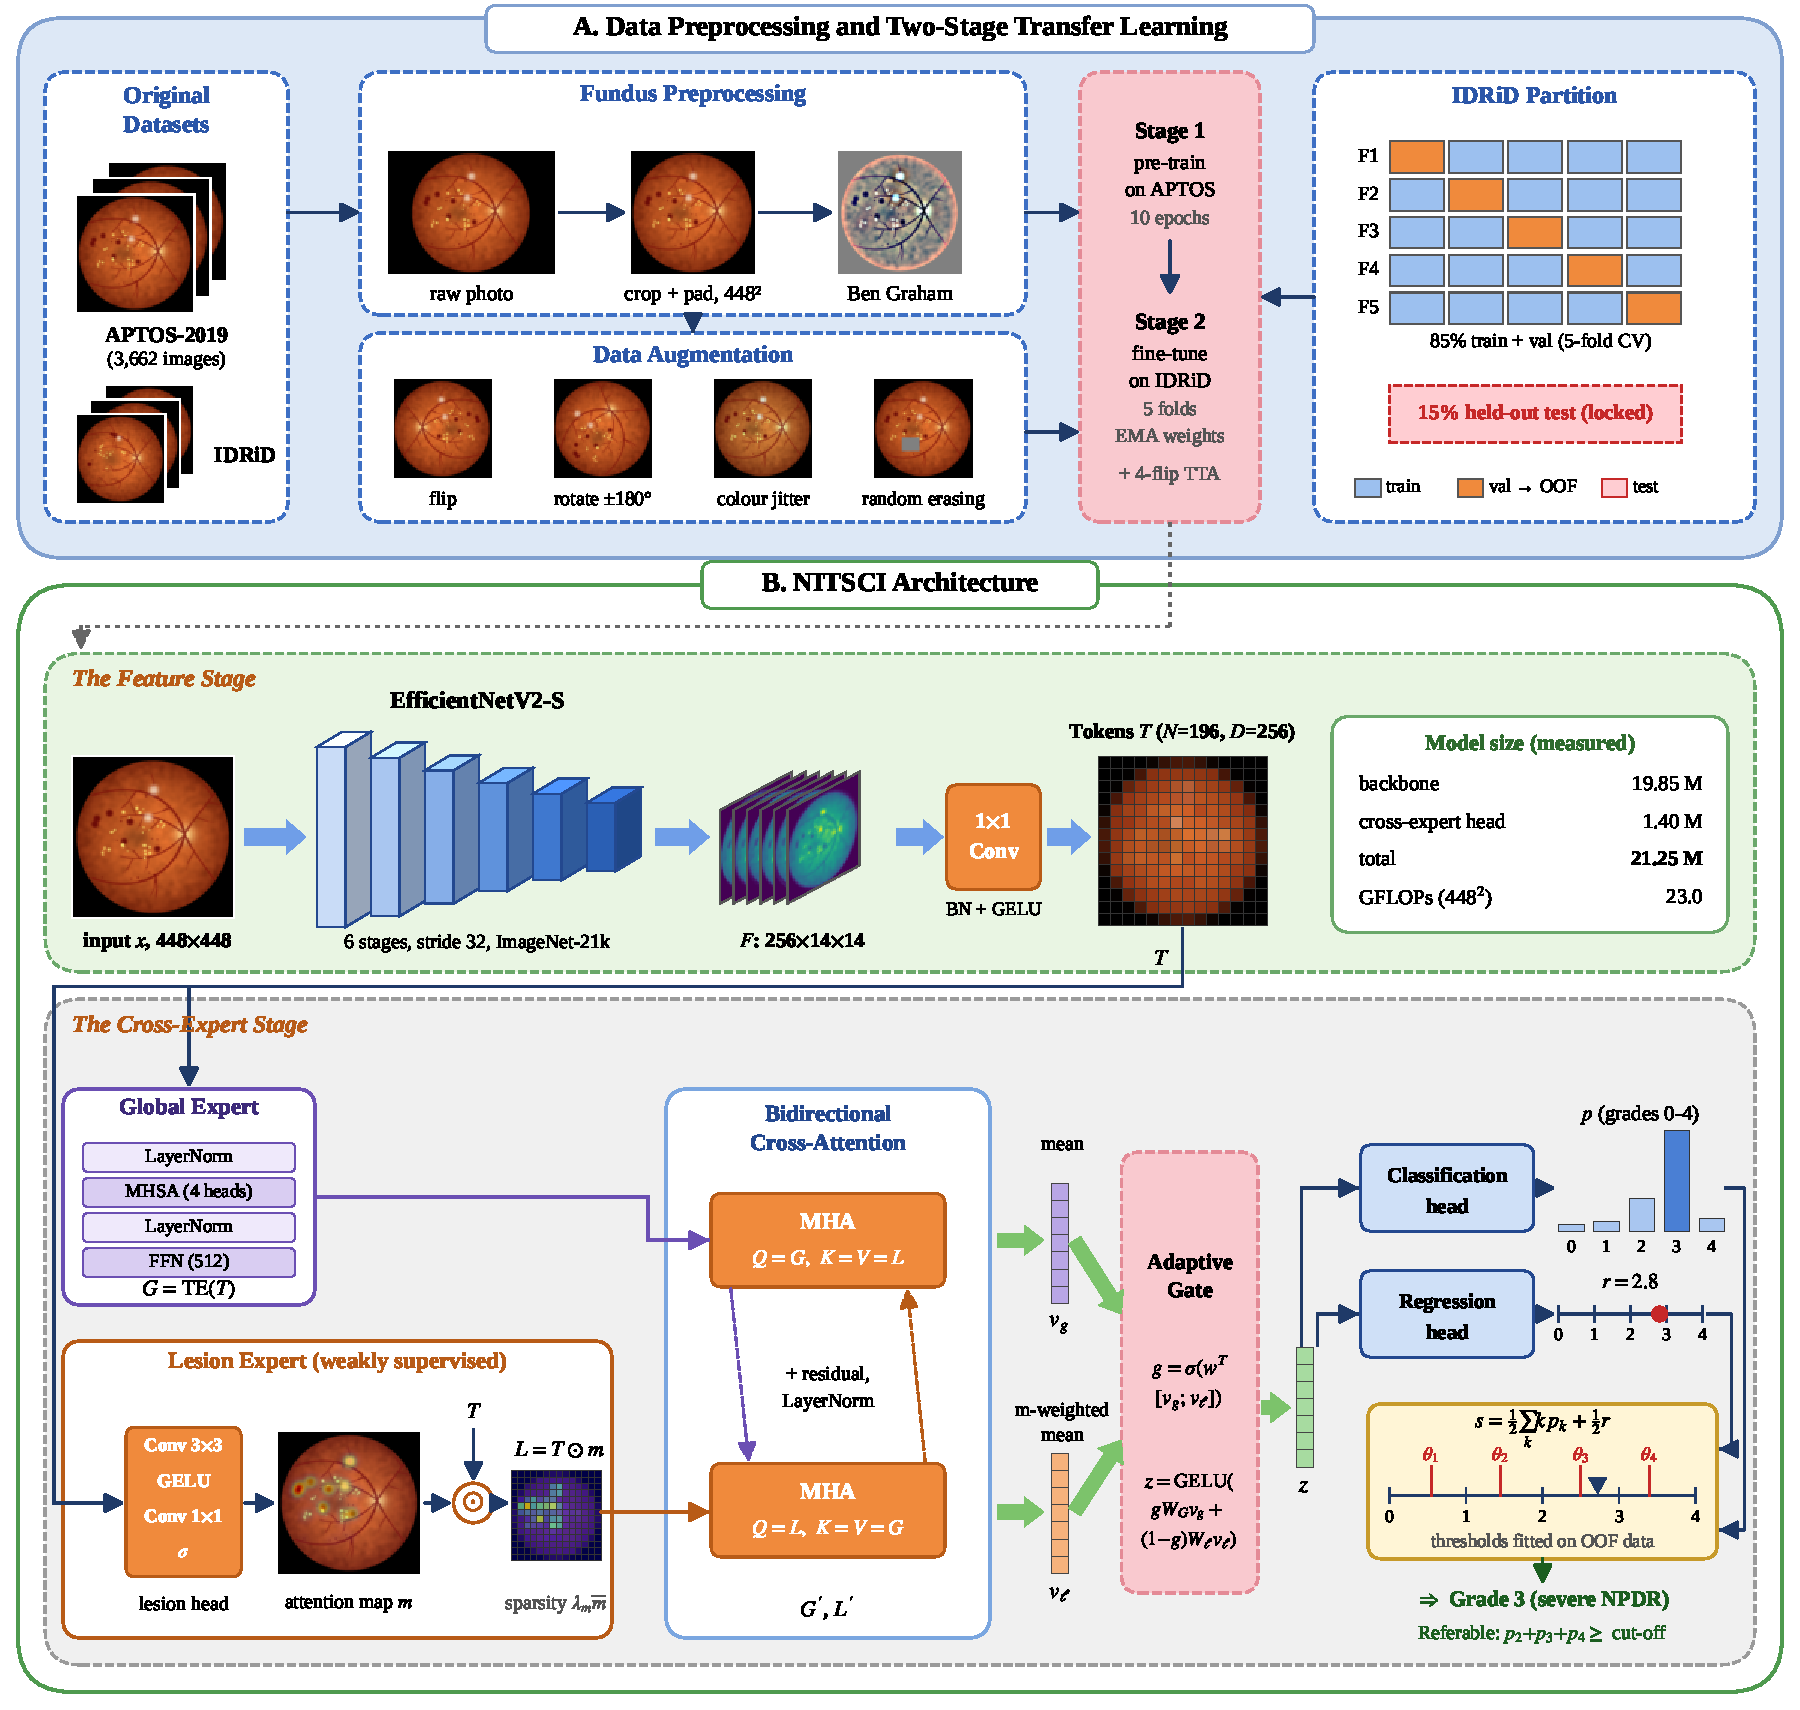
\includegraphics[width=\linewidth]{figures/nitsci_method.pdf}
\caption{Overview of the proposed method. \textbf{(A)} Data preparation and two-stage transfer learning: APTOS-2019
and IDRiD images are pre-processed identically; the full model is pretrained on APTOS-2019 (stage 1) and fine-tuned
on five stratified IDRiD folds (stage 2), while a stratified 15\% IDRiD test set is locked away; out-of-fold
predictions fix the decision rule, the grade thresholds $\theta_1,\dots,\theta_4$ and the referral cut-off.
\textbf{(B)} NITSCI architecture: EfficientNetV2-S features are projected to $N=196$ tokens, processed by a global
expert and by a lesion expert $L=T\odot m$ built from a learned lesion map $m$, coupled by bidirectional
cross-attention, pooled and fused by an adaptive gate $g$; classification and regression heads are combined into the
grade score $s$, whose thresholds come from panel A. Fundus photographs, feature maps and the probability
values shown are synthetic illustrations, not patient data or model outputs.}
\label{fig:arch}
\end{figure}

\subsection{Backbone and tokenisation}
We use EfficientNetV2-S \citep{tan2021efficientnetv2} pretrained on ImageNet-21k and fine-tuned on ImageNet-1k
\citep{ridnik2021imagenet21k}, taken from the \texttt{timm} library \citep{wightman2019timm}. Its last stage
(stride 32, 256 channels) gives a $14\times14$ map for a $448\times448$ input. A $1\times1$ convolution with batch
normalisation and GELU projects it to $F\in\mathbb{R}^{D\times h\times w}$ with $D=256$, which is flattened into
$N=hw=196$ tokens $T\in\mathbb{R}^{N\times D}$.

\subsection{Lesion-attention map and lesion expert}
A light head ($3\times3$ convolution to $D/4$ channels, GELU, $1\times1$ convolution to one channel, sigmoid)
predicts a spatial map $m\in[0,1]^{h\times w}$. No lesion annotation is used: $m$ is learned end-to-end from grade
labels and is encouraged to be sparse by an $\ell_1$ penalty (Eq.~\ref{eq:loss}). The lesion expert is the
re-weighted token set
\begin{equation}
L = T\odot m, \qquad L_i = m_i\,T_i,\; i=1,\dots,N.
\end{equation}

\subsection{Global expert}
The global expert is one pre-norm Transformer encoder layer \citep{vaswani2017attention} with four heads, a
feed-forward width of $2D$ and dropout 0.1, applied to all tokens: $G = \mathrm{TE}(T)$. It models context across
the whole retina, such as the spatial spread of lesions and their relation to the optic disc and macula.

\subsection{Bidirectional cross-attention}
Each expert queries the other with multi-head attention (four heads, dropout 0.1):
\begin{align}
Z_g &= \mathrm{MHA}(Q{=}G,\;K{=}L,\;V{=}L), & G' &= \mathrm{LN}(G + Z_g),\\
Z_\ell &= \mathrm{MHA}(Q{=}L,\;K{=}G,\;V{=}G), & L' &= \mathrm{LN}(L + Z_\ell).
\end{align}
The global stream thus gathers lesion evidence, and the lesion stream receives the context needed to interpret it.

\subsection{Pooling and adaptive gate}
The global stream is mean-pooled, $v_g = \frac1N\sum_i G'_i$, and the lesion stream is pooled with the lesion
weights, $v_\ell = \sum_i m_i L'_i \big/ (\sum_i m_i + \epsilon)$. A scalar gate decides, per image, how much each
expert contributes:
\begin{equation}
g = \sigma\!\left(w^\top[v_g; v_\ell] + b\right),\qquad
z = \mathrm{GELU}\!\left(g\,W_G v_g + (1-g)\,W_L v_\ell\right).
\label{eq:gate}
\end{equation}
This is a two-expert soft mixture \citep{jacobs1991adaptive}; $g$ is also reported for interpretability.

\subsection{Dual head and grade score}
Two heads share $z$: a classification head (LayerNorm, dropout 0.3, linear) gives logits and probabilities
$p\in\Delta^{4}$, and a regression head of the same form gives $r = f_r(z) + 2$, centred on the middle grade.
Their outputs are combined into a continuous score
\begin{equation}
s = \tfrac12\,\textstyle\sum_{k=0}^{4} k\,p_k + \tfrac12\,r .
\label{eq:score}
\end{equation}
A grade is obtained by comparing $s$ with four ordered thresholds $\theta_1<\dots<\theta_4$:
$\hat y = \#\{j:\ s \geq \theta_j\}$.

\subsection{Training objective}
For a mini-batch the loss is
\begin{equation}
\mathcal{L} = \mathrm{CE}_{w,\varepsilon}(p, y) + \lambda_r\,\mathrm{SmoothL1}(r, y) + \lambda_m\,\overline{m},
\label{eq:loss}
\end{equation}
where $\mathrm{CE}_{w,\varepsilon}$ is cross-entropy with label smoothing $\varepsilon = 0.05$
\citep{szegedy2016rethinking} and class weights $w_c \propto n_c^{-1/2}$ (normalised to mean one, computed on the
training fold), $\overline m$ is the mean of the up-sampled lesion map, $\lambda_r = 0.5$ and $\lambda_m = 0.01$.
The square-root weighting is a compromise between ignoring and fully inverting the imbalance.

\subsection{Two-stage training}
\textbf{Stage 1 (APTOS).} The full model, initialised from ImageNet-21k backbone weights, is trained on APTOS-2019 for
10 epochs (learning rate $3\times10^{-4}$, EMA decay 0.999). \textbf{Stage 2 (IDRiD).} For each of the five folds, a
model initialised from the stage-1 weights is fine-tuned for at most 25 epochs (learning rate $2\times10^{-4}$, EMA
decay 0.99, early stopping with patience 8). In both stages we use AdamW \citep{loshchilov2019decoupled} with weight
decay $10^{-4}$, a backbone learning rate one third of the head learning rate, a one-cycle cosine schedule with 10\%
warm-up \citep{smith2019super}, mixed precision \citep{micikevicius2018mixed}, gradient clipping at norm 2, and an
exponential moving average (EMA) of weights \citep{polyak1992acceleration} that is used for validation and saved.
The checkpoint with the highest sum of validation accuracy and quadratic weighted kappa (fixed thresholds
$0.5,1.5,2.5,3.5$, no TTA) is kept.

\subsection{Inference and decision rule}\label{sec:decision}
Each fold model predicts every test image under four views (identity, horizontal flip, vertical flip, both);
probabilities and regression outputs are averaged over views and over the five folds (20 predictions per image).
The decision rule is chosen \emph{on out-of-fold (OOF) predictions only} among three candidates: (i) argmax of $p$;
(ii) rounding $s$ with thresholds $0.5,1.5,2.5,3.5$; (iii) optimised thresholds, found by coordinate search
(four rounds, 80 candidate values per threshold, constrained to remain ordered) maximising OOF accuracy. The chosen
rule was \emph{\res{rule}}, with thresholds (\res{thr}).

\textbf{Referable DR.} For the screening task we use $P(\text{referable}) = p_2 + p_3 + p_4$ and select its
operating threshold on OOF predictions by maximising Youden's $J$ \citep{youden1950index} (selected value
\res{refthr}).

\subsection{Model size and cost}
Table~\ref{tab:cost} lists the parameter counts and floating-point operations, measured with PyTorch
\citep{paszke2019pytorch} on a single $448\times448$ input. The cross-expert head adds 7\% to the parameters of the
backbone.

\begin{table}[!htbp]
\centering\small
\caption{Model size and cost for one $448\times448$ image (FLOPs counted as $2\times$ multiply--accumulates).}
\label{tab:cost}
\begin{tabular}{@{}lcc@{}}
\toprule
Component & Parameters (M) & Notes\\
\midrule
EfficientNetV2-S feature extractor & 19.85 & 256 output channels\\
Cross-expert head (all modules after the backbone) & 1.40 & $D=256$, 4 heads\\
\textbf{NITSCI total} & \textbf{21.25} & 23.0 GFLOPs\\
Plain baseline (same backbone, GAP, same dual head) & 19.92 & --\\
\midrule
Inference latency per image (fp16, batch 16, \res{gpu}) & \multicolumn{2}{l}{\res{mspi} ms per model and view}\\
\bottomrule
\end{tabular}
\end{table}
\sectionend{method}

\sectionbreak
% ---------------- sections/05_experimental_setup.tex ----------------
% =====================================================================
\section{Experimental setup}\label{sec:setup}
% =====================================================================
\subsection{Implementation details}
All experiments were implemented in PyTorch \citep{paszke2019pytorch} with the \texttt{timm} model library
\citep{wightman2019timm} and scikit-learn \citep{pedregosa2011scikit}, and run on a single \res{gpu} GPU. Mixed
precision (fp16) \citep{micikevicius2018mixed} was used for training and inference, and Grad-CAM maps were computed
with the \texttt{pytorch-grad-cam} library \citep{gildenblat2021gradcam}. Random seeds were fixed to 42 for
data splitting and pretraining and to $42+k$ for fold $k$. Table~\ref{tab:hparams} lists all hyper-parameters; none of
them was tuned on the test set. After early stopping, the number of epochs actually run in the five folds was
(\res{epochsrun}).

\begin{table}[!htbp]
\centering\small
\caption{Training and inference hyper-parameters. Values marked $\dagger$ are shared by both stages.}
\label{tab:hparams}
\begin{adjustbox}{max width=\linewidth}
\begin{tabular}{@{}lll@{}}
\toprule
Setting & Stage 1 (APTOS-2019) & Stage 2 (IDRiD, per fold)\\
\midrule
Initialisation & ImageNet-21k backbone & stage-1 weights\\
Epochs (max.) & 10 & 25, early stopping (patience 8)\\
Peak learning rate (head / backbone) & $3\times10^{-4}$ / $1\times10^{-4}$ & $2\times10^{-4}$ / $6.7\times10^{-5}$\\
EMA decay & 0.999 & 0.99\\
Optimiser$^\dagger$ & \multicolumn{2}{l}{AdamW \citep{loshchilov2019decoupled}, weight decay $10^{-4}$}\\
Schedule$^\dagger$ & \multicolumn{2}{l}{one-cycle cosine, 10\% warm-up \citep{smith2019super}}\\
Batch size$^\dagger$ & \multicolumn{2}{l}{16; gradient clipping at $\ell_2$ norm 2.0}\\
Input size$^\dagger$ & \multicolumn{2}{l}{$448\times448$, Ben Graham pre-processing}\\
Loss weights$^\dagger$ & \multicolumn{2}{l}{$\lambda_r=0.5$ (ordinal), $\lambda_m=0.01$ (sparsity), label smoothing 0.05}\\
Class weights$^\dagger$ & \multicolumn{2}{l}{$w_c\propto n_c^{-1/2}$, normalised to mean 1, computed on training data}\\
Checkpoint selection$^\dagger$ & \multicolumn{2}{l}{max.\ validation accuracy + QWK (EMA weights, fixed cut-points, no TTA)}\\
Inference & -- & 5 fold models $\times$ 4 flips = 20 predictions per image\\
\bottomrule
\end{tabular}
\end{adjustbox}
\end{table}

\subsection{Evaluation metrics}
Let $y_i$ and $\hat y_i$ be the reference and predicted grades of test image $i$, $i=1,\dots,n$, and let $O$ be the
$5\times5$ confusion matrix with entries $O_{jk}$ counting images of grade $j$ predicted as grade $k$.

\paragraph{Five-class grading.} \emph{Accuracy} is the fraction of exactly correct grades. Because the classes are
imbalanced, we also report \emph{balanced accuracy}, the mean of the per-class recalls, and the macro-averaged
precision, recall and F1, which weight every grade equally. The \emph{quadratic weighted kappa}
\citep{cohen1968weighted} measures agreement beyond chance while penalising errors by the squared grade distance:
\begin{equation}
\kappa_w = 1 - \frac{\sum_{j,k} W_{jk}\,O_{jk}}{\sum_{j,k} W_{jk}\,E_{jk}},\qquad
W_{jk} = \frac{(j-k)^2}{(K-1)^2},
\end{equation}
where $E$ is the expected confusion matrix under independence (outer product of the marginal histograms, scaled to
$n$) and $K=5$. We also report unweighted Cohen's kappa, the Matthews correlation coefficient (MCC), the
\emph{within-one-grade accuracy} $\frac1n\sum_i \mathbb{1}[|y_i-\hat y_i|\le1]$, which quantifies how many errors are
between adjacent grades, and macro one-vs-rest ROC AUC and average precision computed from the ensemble
probabilities.

\paragraph{Referable DR.} With TP, FN, FP and TN counted for the binary task (grade $\geq2$ vs.\ $<2$), we report
sensitivity $\mathrm{TP}/(\mathrm{TP}+\mathrm{FN})$, specificity $\mathrm{TN}/(\mathrm{TN}+\mathrm{FP})$, positive and
negative predictive values, accuracy, F1 and the threshold-free ROC AUC of $P(\text{referable})$. Sensitivity is the
clinically most important quantity, because a missed referable case delays treatment.

\subsection{Statistical analysis}
\paragraph{Confidence intervals.} For each test metric we compute a 95\% percentile bootstrap interval
\citep{efron1993introduction}: the $n$ test images are resampled with replacement 2000 times, the metric is recomputed
on each resample, and the 2.5th and 97.5th percentiles are reported. Predictions are fixed during resampling, so the
interval reflects uncertainty due to the finite test set, not training randomness.

\paragraph{Paired comparisons.} All configurations are evaluated on the same test images, so we compare each
ablation with the full model using the two-sided exact McNemar test on per-image correctness
\citep{dietterich1998approximate}. If $b$ images are correct only for the full model and $c$ only for the ablation,
the $p$-value is
\begin{equation}
p = \min\!\Big(1,\; 2\sum_{i=0}^{\min(b,c)} \binom{b+c}{i}\,2^{-(b+c)}\Big).
\end{equation}
We report $p$-values without claiming significance for a single threshold; seven ablations are compared, so a
Bonferroni-adjusted level of $0.05/7\approx0.007$ is the conservative reference.

\paragraph{Cross-validation estimates.} We additionally report OOF metrics and their mean and standard deviation across
folds. These are slightly optimistic, because each fold's checkpoint is selected on the same fold
\citep{varma2006bias}; they are given for completeness and are not used as the main result.

\subsection{Compared configurations}
All configurations use identical splits, seeds, augmentation, schedule and inference, and differ in one factor only:
\begin{itemize}
\item \textbf{Plain}: the same backbone and $1\times1$ projection, followed by global average pooling and the same
  dual head and loss. This is the standard transfer-learning baseline and isolates the effect of the whole
  cross-expert head.
\item \textbf{w/o APTOS}: no stage-1 pretraining; the model is initialised from ImageNet-21k only.
\item \textbf{CLAHE}: CLAHE + bilateral filtering instead of Ben Graham pre-processing, with stage 1 repeated.
\item \textbf{w/o ordinal head}: $\lambda_r=0$; the regression output is untrained, and the decision-rule selection on OOF
  data (Section~\ref{sec:decision}) decides whether the score $s$ or the argmax of $p$ is used.
\item \textbf{w/o lesion map}: $m\equiv1$; the lesion expert receives all tokens with equal weight.
\item \textbf{w/o cross-attention}: the experts are only normalised, $G'=\mathrm{LN}(G)$, $L'=\mathrm{LN}(L)$.
\item \textbf{w/o gate}: the gate is fixed to $g=0.5$, i.e.\ equal contribution of both experts.
\end{itemize}
For the architectural variants, stage 1 is repeated so that pretraining and fine-tuning use the same architecture.

\subsection{Reproducibility}
The notebook, the export cell that writes every reported number and figure, the ablation variants and the script that
inserts the numbers into this manuscript are released together (see Code availability). The held-out test indices and
per-image predictions are stored in the exported results, so every table can be regenerated and every comparison
re-tested without retraining.
\sectionend{setup}

\sectionbreak
% ---------------- sections/06_results.tex ----------------
% =====================================================================
\section{Results}\label{sec:results}
% =====================================================================
This section reports the held-out test results for five-class grading (Section~\ref{sec:res5}) and referable-DR
screening (Section~\ref{sec:resref}), followed by the ablation study, the effect of inference-time choices, training
behaviour, visual explanations and computational cost. Unless stated otherwise, all numbers refer to the
\res{ntest}-image IDRiD test set and to the five-fold ensemble with test-time augmentation.

\subsection{Five-class grading}\label{sec:res5}
Table~\ref{tab:main} reports the held-out test performance. Cross-validation estimates on the training portion are
given for comparison: OOF accuracy \res{oofacc}\% and QWK \res{oofqwk} (per-fold accuracy \res{foldacc}\%, per-fold
QWK \res{foldqwk}).

\begin{table}[!htbp]
\centering\small
\caption{Five-class DR grading on the held-out IDRiD test set ($n=\res{ntest}$). Ensemble of five fold models with
four-view TTA, decision rule chosen on OOF data. Brackets: 95\% bootstrap CI.}
\label{tab:main}
\begin{adjustbox}{max width=\linewidth}
\begin{tabular}{@{}lc@{\hspace{2.2em}}lc@{}}
\toprule
Metric & Value & Metric & Value\\
\midrule
Accuracy (\%) & \res{acc5} \res{acc5ci} & Macro precision (\%) & \res{precmacro5}\\
Balanced accuracy (\%) & \res{bacc5} & Macro recall (\%) & \res{recmacro5}\\
Quadratic weighted kappa & \res{qwk5} \res{qwk5ci} & Macro F1 (\%) & \res{f1macro5} \res{f1macro5ci}\\
Cohen's kappa & \res{kappa5} & Weighted F1 (\%) & \res{f1w5}\\
MCC & \res{mcc5} & Within-one-grade accuracy (\%) & \res{within1}\\
Macro ROC AUC (OvR) & \res{auc5} & Macro average precision & \res{ap5}\\
\bottomrule
\end{tabular}
\end{adjustbox}
\end{table}

\begin{table}[!htbp]
\centering\small
\caption{Per-grade precision, recall and F1 (\%) on the test set.}
\label{tab:perclass}
\begin{tabular}{@{}lccccc@{}}
\toprule
 & 0 No DR & 1 Mild & 2 Moderate & 3 Severe & 4 PDR\\
\midrule
Support & \res{nte0} & \res{nte1} & \res{nte2} & \res{nte3} & \res{nte4}\\
Precision & \res{p0} & \res{p1} & \res{p2} & \res{p3} & \res{p4}\\
Recall & \res{r0} & \res{r1} & \res{r2} & \res{r3} & \res{r4}\\
F1 & \res{f0} & \res{f1} & \res{f2} & \res{f3} & \res{f4}\\
\bottomrule
\end{tabular}
\end{table}

Table~\ref{tab:perclass} and Fig.~\ref{fig:cm}(a) show where errors occur.
\authnote{Describe the confusion pattern: e.g.\ whether most errors are between adjacent grades (consistent with
within-one-grade accuracy of \res{within1}\%), and which grade is weakest. Grade 1 is typically hardest because it
is defined by microaneurysms only.}



\subsection{Referable DR screening}\label{sec:resref}
Table~\ref{tab:ref} reports the screening task. The operating threshold was fixed on OOF data before the test set was
evaluated; the OOF AUC was \res{oofrefauc}. Figure~\ref{fig:cm} (right) shows the ROC curves.

\begin{table}[!htbp]
\centering\small
\caption{Referable DR (grade $\geq 2$ vs.\ $<2$) on the held-out test set. Brackets: 95\% bootstrap CI.}
\label{tab:ref}
\begin{tabular}{@{}lc@{\hspace{2.2em}}lc@{}}
\toprule
Metric & Value & Metric & Value\\
\midrule
ROC AUC & \res{refauc} \res{refaucci} & PPV (\%) & \res{refppv}\\
Sensitivity (\%) & \res{refsens} \res{refsensci} & NPV (\%) & \res{refnpv}\\
Specificity (\%) & \res{refspec} \res{refspecci} & F1 (\%) & \res{reff1}\\
Accuracy (\%) & \res{refacc} \res{refaccci} & TP / FN / FP / TN & \res{tp} / \res{fn} / \res{fp} / \res{tn}\\
\bottomrule
\end{tabular}
\end{table}

\begin{figure}[!htbp]
\centering
\begin{minipage}[c]{0.6\linewidth}\centering
\fig[0.4]{confusion.pdf}{\linewidth}{Confusion matrices (5-class and referable).}
\end{minipage}\hfill
\begin{minipage}[c]{0.37\linewidth}\centering
\fig[0.9]{roc.pdf}{\linewidth}{ROC curves.}
\end{minipage}
\caption{Held-out test set. Left: confusion matrices for (a) five-class grading and (b) referable DR (grade $\geq2$).
Right: one-vs-rest ROC curves for each grade and for referable DR (bold).}
\label{fig:cm}
\end{figure}

\subsection{Ablation study}
Table~\ref{tab:ablation} compares the full model with the configurations of Section~\ref{sec:setup}. All runs share
the same test images, so the McNemar $p$-value tests whether per-image correctness differs from the full model.

\begin{table}[!htbp]
\centering\small
\caption{Ablation study on the held-out IDRiD test set. Five-class accuracy, QWK and macro F1; referable-DR AUC,
sensitivity and specificity. $p$: exact McNemar test vs.\ the full model on five-class correctness.}
\label{tab:ablation}
\begin{adjustbox}{max width=\linewidth}
\begin{tabular}{@{}lccccccc@{}}
\toprule
Configuration & Params (M) & Acc (\%) & QWK & F1 (\%) & Ref.\ AUC & Sens.\ (\%) & Spec.\ (\%)\\
\midrule
\textbf{NITSCI (full)} & \res{abfullparams} & \res{abfullacc} & \res{abfullqwk} & \res{abfullf1} & \res{abfullrefauc} & \res{abfullrefsens} & \res{abfullrefspec}\\
\midrule
Plain (GAP head) & \res{abplainparams} & \res{abplainacc} & \res{abplainqwk} & \res{abplainf1} & \res{abplainrefauc} & \res{abplainrefsens} & \res{abplainrefspec}\\
w/o APTOS pretraining & \res{abnoaptosparams} & \res{abnoaptosacc} & \res{abnoaptosqwk} & \res{abnoaptosf1} & \res{abnoaptosrefauc} & \res{abnoaptosrefsens} & \res{abnoaptosrefspec}\\
CLAHE pre-processing & \res{abclaheparams} & \res{abclaheacc} & \res{abclaheqwk} & \res{abclahef1} & \res{abclaherefauc} & \res{abclaherefsens} & \res{abclaherefspec}\\
w/o ordinal head & \res{abnoregparams} & \res{abnoregacc} & \res{abnoregqwk} & \res{abnoregf1} & \res{abnoregrefauc} & \res{abnoregrefsens} & \res{abnoregrefspec}\\
w/o lesion map & \res{abnolesionparams} & \res{abnolesionacc} & \res{abnolesionqwk} & \res{abnolesionf1} & \res{abnolesionrefauc} & \res{abnolesionrefsens} & \res{abnolesionrefspec}\\
w/o cross-attention & \res{abnocrossparams} & \res{abnocrossacc} & \res{abnocrossqwk} & \res{abnocrossf1} & \res{abnocrossrefauc} & \res{abnocrossrefsens} & \res{abnocrossrefspec}\\
w/o adaptive gate & \res{abnogateparams} & \res{abnogateacc} & \res{abnogateqwk} & \res{abnogatef1} & \res{abnogaterefauc} & \res{abnogaterefsens} & \res{abnogaterefspec}\\
\bottomrule
\end{tabular}
\end{adjustbox}

\vspace{3pt}
\parbox{\linewidth}{\footnotesize McNemar $p$ vs.\ full: Plain \res{abplainp}; w/o APTOS \res{abnoaptosp}; CLAHE \res{abclahep};
w/o ordinal \res{abnoregp}; w/o lesion map \res{abnolesionp}; w/o cross-attention \res{abnocrossp};
w/o gate \res{abnogatep}.
Parameter counts of ``w/o cross-attention'' and ``w/o gate'' include the unused modules, which are kept so that
the remaining weights are initialised identically.}
\end{table}

\authnote{Interpret Table~\ref{tab:ablation} honestly: name the components whose removal lowers accuracy/QWK by
more than the width of the bootstrap interval or with McNemar $p<0.05$, and state plainly which components show no
measurable effect at this test-set size. Do not claim a component ``improves'' performance if its $p$-value is
large.}

\subsection{Inference-time choices}
Table~\ref{tab:infer} isolates the effect of the decision rule, TTA and fold ensembling without retraining. The
decision rule was selected on OOF accuracy; test values are shown only to document the outcome of that choice.

\begin{table}[!htbp]
\centering\small
\caption{Effect of inference-time choices. Top: decision rules (OOF accuracy was used for selection). Bottom:
single fold models vs.\ ensemble, with and without TTA (mean $\pm$ SD over five folds for single models).}
\label{tab:infer}
\begin{tabular}{@{}lccc@{}}
\toprule
Decision rule & OOF acc.\ (\%) & Test acc.\ (\%) & Test QWK\\
\midrule
Argmax of $p$ & \res{oofargmax} & \res{testargmax} & \res{testargmaxqwk}\\
Rounded score $s$ & \res{oofrounded} & \res{testrounded} & \res{testroundedqwk}\\
Optimised thresholds on $s$ & \res{oofopt} & \res{testopt} & \res{testoptqwk}\\
\bottomrule
\end{tabular}

\medskip
\begin{tabular}{@{}lcc@{}}
\toprule
Prediction & Test acc.\ (\%) & Test QWK\\
\midrule
Single fold, TTA & \res{singleacc} & \res{singleqwk}\\
5-fold ensemble, no TTA & \res{notaacc} & \res{notaqwk}\\
5-fold ensemble + TTA & \res{ttaacc} & \res{ttaqwk}\\
\bottomrule
\end{tabular}
\end{table}

\subsection{Training behaviour}
Supplementary Fig.~\ref{fig:curves} shows the training loss and validation metrics for each fold. \authnote{Comment on
convergence, the epoch at which early stopping triggered, and the spread between folds.}



\subsection{Visual explanations}
Figure~\ref{fig:explain} shows Grad-CAM maps for the predicted grade and the learned lesion-attention map $m$ for test
images, together with the gate value $g$ (Eq.~\ref{eq:gate}). Because $m$ is learned without lesion annotations, these
maps are qualitative only; we do not claim that they localise lesions. \authnote{Describe what the maps show, e.g.\
whether high attention falls on haemorrhages or exudates, and whether $g$ differs between low and high grades. A
quantitative check against the IDRiD lesion masks (e.g.\ pointing-game accuracy) would strengthen this section.}

\begin{figure}[!htbp]
\centering
\fig[0.75]{explain.png}{0.6\linewidth}{Original image, Grad-CAM, lesion attention for four test images.}
\caption{Test images (top), Grad-CAM for the predicted grade (middle), and the learned lesion-attention map with
gate value $g$ (bottom), from the fold-1 model.}
\label{fig:explain}
\end{figure}

\subsection{Computational cost}
The full model has 21.25\,M parameters and requires 23.0\,GFLOPs per $448\times448$ image (Table~\ref{tab:cost}).
Measured inference time on the \res{gpu} was \res{mspi}\,ms per image per model and view, so the 20-prediction
ensemble costs about twenty times this value per image. \authnote{State whether this is acceptable for screening
throughput, and note that a single fold model without TTA is the cheaper option whose accuracy is given in
Table~\ref{tab:infer}.}

\sectionend{results}

\sectionbreak
% ---------------- sections/07_discussion.tex ----------------
% =====================================================================
\section{Discussion}\label{sec:discussion}
% =====================================================================
\subsection{Main findings}
On a held-out IDRiD test set that played no role in any modelling decision, NITSCI reached a five-class accuracy of
\res{acc5}\% with a QWK of \res{qwk5}, graded \res{within1}\% of images within one level of the reference, and
detected referable DR with an AUC of \res{refauc} at a sensitivity of \res{refsens}\% and a specificity of
\res{refspec}\%. \authnote{Summarise in two or three sentences, using only claims supported by
Tables~\ref{tab:main}--\ref{tab:infer}: (1) whether the full model improves on the plain baseline beyond the bootstrap
interval; (2) which ablations had the largest effect; (3) whether the ordinal head and threshold fitting reduced large
errors, visible in QWK and within-one-grade accuracy.}

\subsection{Interpretation of the components}
\paragraph{Cross-dataset pretraining.} APTOS-2019 differs from IDRiD in cameras, image quality and population, but
shares the grading scale and the visual vocabulary of DR lesions. Pretraining on it exposes the model to roughly eight
times more graded fundus images before it sees IDRiD, which is consistent with the general observation that
in-domain data narrows the gap left by ImageNet pretraining \citep{raghu2019transfusion}. \authnote{Report the size of
the ``w/o APTOS'' effect from Table~\ref{tab:ablation} and whether it is the largest single factor.}

\paragraph{Lesion expert, cross-attention and gate.} The three architectural components address the same problem from
different angles: the lesion map concentrates the representation on a few informative locations, cross-attention
lets lesion tokens be interpreted in their retinal context, and the gate allows the balance between global and lesion
evidence to vary from image to image. A plausible expectation is that the gate favours lesion evidence for borderline
images between grades 0, 1 and 2, where the decision depends on a few lesions, and global context for advanced
disease, where lesions are widespread. \authnote{Check this with the gate values exported for the test images, or
remove the sentence. Report which of the three ablations changed accuracy or QWK beyond the confidence interval,
and say plainly if a component had no measurable effect at this test-set size.}

\paragraph{Ordinal head and decision rule.} Combining the expected grade of the classifier with a regression output
produces a score that changes smoothly with disease severity, so errors tend to fall on adjacent grades. Fitting the
cut-points on out-of-fold predictions adapts them to the class balance of IDRiD without touching the test set. The
comparison of decision rules in Table~\ref{tab:infer} shows how much of the final accuracy is due to the rule rather
than to the network. \authnote{Comment on whether the OOF ranking of the rules matched their test ranking; if not,
this indicates that the threshold fit partly reflects noise in a small OOF set.}

\paragraph{Ensembling and TTA.} Averaging 20 predictions per image reduces variance, which matters most for the
under-represented grades. The difference between a single fold model and the ensemble (Table~\ref{tab:infer}) also
quantifies a practical trade-off: a single model without TTA is twenty times cheaper at inference.

\subsection{Comparison with published results}
Direct numerical comparison with the IDRiD grading challenge \citep{porwal2020idrid} is not possible from this study,
because the challenge uses an official train/test partition whereas we use a stratified random hold-out of the Kaggle
copy. Numbers reported on different splits, with different pre-processing and sometimes with thresholds tuned on the
test set, are not comparable, and placing them in the same table would mislead the reader. We therefore compare
against a plain baseline and ablations trained under identical conditions (Table~\ref{tab:ablation}).
\authnote{Either (a) re-run the pipeline on the official IDRiD grading partition and add a table comparing with the
challenge results reported in \citet{porwal2020idrid}, copying the numbers from that paper; or (b) keep this paragraph.}

\subsection{Interpretability}
The lesion-attention map and Grad-CAM \citep{selvaraju2017gradcam} offer a view of where the model looks, which can help
clinicians to spot obvious failure modes. They should not be over-interpreted: saliency maps can be insensitive to the
model parameters \citep{adebayo2018sanity}, and post-hoc explanations of black-box models are not a substitute for
validated, inherently interpretable evidence in high-stakes decisions \citep{rudin2019stop}. Because our lesion map is
learned without lesion masks, we treat it as a qualitative aid only; validating it against the IDRiD lesion
annotations is part of future work.

\subsection{Limitations}
\begin{itemize}
\item \textbf{Small test set.} With \res{ntest} test images, confidence intervals are wide, and per-grade metrics for
  rare grades rest on few images. Differences of a few percentage points between configurations may not be
  statistically detectable.
\item \textbf{Single target dataset.} All results come from IDRiD, collected at one centre with one camera.
  Performance on other populations, cameras and image-quality levels, for example Messidor
  \citep{decenciere2014messidor} or DDR \citep{li2019ddr}, has not been tested.
\item \textbf{Non-official split.} The random hold-out prevents direct comparison with the IDRiD challenge.
\item \textbf{Weakly supervised lesion map.} The lesion-attention map has not been validated against lesion masks.
\item \textbf{Training randomness.} Variance is reflected through five folds but not through repeated runs with
  different seeds.
\item \textbf{Reference standard.} Grades are taken from the dataset providers; grader variability, which is
  substantial for DR \citep{krause2018grader}, is not modelled.
\item \textbf{Optimistic OOF estimates.} Checkpoints are selected on the same folds used for OOF predictions, so the
  cross-validation numbers (but not the test numbers) are slightly optimistic \citep{varma2006bias}.
\end{itemize}

\subsection{Ethical and clinical considerations}
NITSCI is a research prototype, not a medical device. Both datasets are public and de-identified. Several issues must
be addressed before any clinical use. First, models trained on data from one population can perform worse, or fail
silently, on others; algorithmic bias in health care has had measurable consequences \citep{obermeyer2019dissecting},
so subgroup performance by age, sex, ethnicity and camera should be reported. Second, the operating point should be
set together with clinicians to reach a target sensitivity rather than to maximise accuracy, since a false negative
delays treatment while a false positive costs a specialist visit. Third, probabilities from deep networks are often
mis-calibrated \citep{guo2017calibration}; calibration should be checked before a probability threshold is used for
referral. Finally, prospective external validation reported according to TRIPOD+AI \citep{collins2024tripod} is
required, as autonomous DR systems in clinical use have shown \citep{abramoff2018pivotal}.
\sectionend{discussion}

\sectionbreak
% ---------------- sections/08_conclusion.tex ----------------
% =====================================================================
\section{Conclusion and future work}\label{sec:conclusion}
% =====================================================================
\subsection{Conclusion}
This paper presented NITSCI, a compact network for five-level diabetic retinopathy grading from colour fundus
photographs, designed for the common situation in which only a few hundred labelled images are available. The model
places a cross-expert head of 1.40\,M parameters on an EfficientNetV2-S backbone. A global expert relates all retinal
regions through self-attention; a lesion expert receives the same features re-weighted by a lesion-attention map that
is learned from grade labels alone; the two experts exchange information through bidirectional cross-attention; and
an image-adaptive gate decides how much each contributes. A classification head and an ordinal regression head are
combined into one continuous grade score, so that the decision respects the order of the ICDR scale.

The second contribution is the evaluation protocol. The model is pretrained on APTOS-2019, fine-tuned on IDRiD with
stratified five-fold cross-validation, and applied as a twenty-member ensemble of fold models and flips. Every
data-dependent decision, including the choice of decision rule, the four grade cut-points and the referral threshold,
is made on out-of-fold predictions. The held-out test set is used once, and every result is reported with a bootstrap
confidence interval; every ablation is compared with the full model by a paired exact test. This protocol avoids the
optimistic bias that arises when thresholds or models are selected on the test set, a frequent problem in small
medical datasets.

Under this protocol NITSCI achieved a five-class accuracy of \res{acc5}\% (95\% CI \res{acc5ci}) with a quadratic
weighted kappa of \res{qwk5}, and a referable-DR AUC of \res{refauc} with sensitivity \res{refsens}\% and specificity
\res{refspec}\% on the IDRiD test set. \authnote{One or two sentences on the most important ablation findings, for
example the effect of APTOS pretraining and of the cross-expert head relative to the plain baseline, stated with their
confidence intervals or $p$-values.} These results indicate that careful use of a larger in-domain dataset, an
architecture that focuses on lesion evidence without needing lesion annotations, and an ordinal decision rule can
make DR grading on small datasets more reliable. They do not establish clinical readiness, which requires external
and prospective validation.

Table~\ref{tab:summary} links each challenge identified in the Introduction to the component of NITSCI that
addresses it and to the experiment that measures its effect.

\begin{table}[!htbp]
\centering\small
\caption{Summary of the challenges addressed, the corresponding design choices, and where their effect is measured.}
\label{tab:summary}
\begin{tabularx}{\linewidth}{@{}>{\raggedright\arraybackslash}p{3.3cm}>{\raggedright\arraybackslash}X>{\raggedright\arraybackslash}p{3.5cm}@{}}
\toprule
Challenge & Design choice in NITSCI & Evidence\\
\midrule
Small, sparse lesion evidence & Lesion-attention map defining a lesion expert; bidirectional cross-attention with a
  global expert; adaptive gate & Ablations w/o lesion map, w/o cross-attention, w/o gate; plain baseline
  (Table~\ref{tab:ablation})\\
Ordered labels & Classification + ordinal regression heads fused into one score; cut-points fitted on OOF data &
  Ablation w/o ordinal head; decision-rule comparison (Table~\ref{tab:infer}); QWK, within-one-grade accuracy\\
Few labelled images & APTOS-2019 pretraining; EMA weights; five-fold ensemble with TTA & Ablation w/o APTOS;
  single model vs.\ ensemble (Table~\ref{tab:infer})\\
Camera and illumination differences & Ben Graham local-contrast normalisation & Ablation CLAHE
  (Table~\ref{tab:ablation})\\
Class imbalance & Inverse-square-root class weights, label smoothing; balanced metrics & Balanced accuracy, macro F1,
  per-grade results (Table~\ref{tab:perclass})\\
Optimistic evaluation & Test set used once; thresholds on OOF data; bootstrap CIs; McNemar tests &
  Tables~\ref{tab:main}--\ref{tab:ablation}\\
\bottomrule
\end{tabularx}
\end{table}

\subsection{Future work}
Five directions follow directly from the limitations identified in Section~\ref{sec:discussion}:
\begin{enumerate}
\item \textbf{Official partition and benchmark comparison.} Re-running the pipeline on the official IDRiD grading
  partition will allow direct comparison with the challenge results \citep{porwal2020idrid}.
\item \textbf{External validation.} Evaluating the trained ensemble without any re-training on independent datasets
  such as Messidor \citep{decenciere2014messidor} and DDR \citep{li2019ddr}, with subgroup analysis by camera and image
  quality, will measure how well the model generalises.
\item \textbf{Validated lesion attention.} The IDRiD lesion masks make it possible to test whether the learned
  lesion-attention map actually highlights lesions, for example with pointing-game accuracy, and to add weak lesion
  supervision when masks are available \citep{zhou2019collaborative}.
\item \textbf{Stronger initialisation.} Replacing the ImageNet-21k backbone with a retinal foundation model
  \citep{zhou2023foundation} may improve data efficiency further, and the cross-expert head can be attached to any
  backbone that produces a spatial feature map.
\item \textbf{Calibrated, uncertainty-aware referral.} Calibrating the referral probability
  \citep{guo2017calibration} and using the disagreement between ensemble members as an uncertainty signal to
  defer difficult cases to a human grader \citep{araujo2020drgraduate,lakshminarayanan2017simple} would make the system
  safer to deploy in a screening workflow.
\end{enumerate}

\subsection{Recommendations for small-dataset grading studies}
Beyond the specific model, our experience suggests four practices for studies that, like this one, work with a few
hundred labelled images:
\begin{itemize}
\item \textbf{Lock the test set first.} Split it off before any experiment and record its indices; tune nothing on it,
  including thresholds and the choice between decision rules.
\item \textbf{Report uncertainty, not only point estimates.} With fewer than one hundred test images, a bootstrap
  interval is often wider than the differences between methods; reporting it prevents over-claiming.
\item \textbf{Compare under identical conditions.} Baselines and ablations should share splits, pre-processing,
  augmentation and inference; numbers copied from papers that used other splits are not comparable.
\item \textbf{Release the pipeline.} Code that regenerates every number, including the test indices and per-image
  predictions, lets reviewers and other groups verify and extend the results.
\end{itemize}
\sectionend{conclusion}


\clearpage
% =====================================================================
\section*{Declarations}\label{start:decl}
% =====================================================================
\paragraph{CRediT authorship contribution statement.}
\authnote{e.g.\ Name: Conceptualization, Methodology, Software, Investigation, Writing -- original draft.
Name: Supervision, Writing -- review \& editing.}

\paragraph{Declaration of competing interest.}
The authors declare that they have no known competing financial interests or personal relationships that could have
appeared to influence the work reported in this paper.

\paragraph{Funding.} \authnote{Funding source and grant number, or ``This research did not receive any specific grant
from funding agencies in the public, commercial, or not-for-profit sectors.''}

\paragraph{Data availability.}
IDRiD and APTOS-2019 are publicly available from their providers \citep{porwal2018idrid,aptos2019}. The test-set
indices, per-image predictions and all metrics are produced by the released code.

\paragraph{Code availability.}
\authnote{Repository URL (e.g.\ GitHub + Zenodo DOI) containing the notebook, export cell and trained weights.}

\paragraph{Ethics statement.}
This study used only publicly available, de-identified datasets; no new data were collected from human participants.

\paragraph{Declaration of generative AI and AI-assisted technologies in the writing process.}
During the preparation of this work the authors used an AI assistant (Claude, Anthropic) to help draft and structure
the manuscript text from the authors' code. After using this tool, the authors reviewed and edited the content as
needed and take full responsibility for the content of the publication.
\authnote{Keep this statement accurate; most publishers, including Elsevier, require it.}

\paragraph{Acknowledgements.} \authnote{Optional.}

\begin{thebibliography}{80}
\providecommand{\natexlab}[1]{#1}
\providecommand{\url}[1]{\texttt{#1}}
\expandafter\ifx\csname urlstyle\endcsname\relax
  \providecommand{\doi}[1]{doi: #1}\else
  \providecommand{\doi}{doi: \begingroup \urlstyle{rm}\Url}\fi

\bibitem[Yau et~al.(2012)Yau, Rogers, Kawasaki, Lamoureux, Kowalski, Bek, Chen,
  Dekker, Fletcher, Grauslund, et~al.]{yau2012global}
Joanne W.~Y. Yau, Sophie~L. Rogers, Ryo Kawasaki, Ecosse~L. Lamoureux,
  Jonathan~W. Kowalski, Toke Bek, Shih-Jen Chen, Jacqueline~M. Dekker, Astrid
  Fletcher, Jakob Grauslund, et~al.
\newblock Global prevalence and major risk factors of diabetic retinopathy.
\newblock \emph{Diabetes Care}, 35\penalty0 (3):\penalty0 556--564, 2012.
\newblock \doi{10.2337/dc11-1909}.

\bibitem[Teo et~al.(2021)Teo, Tham, Yu, Chee, Rim, Cheung, Bikbov, Wang, Tang,
  Lu, et~al.]{teo2021global}
Zhen~Ling Teo, Yih-Chung Tham, Marco Yu, Miao~Li Chee, Tyler~Hyungtaek Rim,
  Ning Cheung, Mukharram~M. Bikbov, Ya~Xing Wang, Yating Tang, Yi~Lu, et~al.
\newblock Global prevalence of diabetic retinopathy and projection of burden
  through 2045: Systematic review and meta-analysis.
\newblock \emph{Ophthalmology}, 128\penalty0 (11):\penalty0 1580--1591, 2021.
\newblock \doi{10.1016/j.ophtha.2021.04.027}.

\bibitem[Ting et~al.(2016)Ting, Cheung, and Wong]{ting2016diabetic}
Daniel Shu~Wei Ting, Gemmy Chui~Ming Cheung, and Tien~Yin Wong.
\newblock Diabetic retinopathy: global prevalence, major risk factors,
  screening practices and public health challenges: a review.
\newblock \emph{Clinical \& Experimental Ophthalmology}, 44\penalty0
  (4):\penalty0 260--277, 2016.
\newblock \doi{10.1111/ceo.12696}.

\bibitem[Wilkinson et~al.(2003)Wilkinson, Ferris, Klein, Lee, Agardh, Davis,
  Dills, Kampik, Pararajasegaram, and Verdaguer]{wilkinson2003proposed}
C.~P. Wilkinson, Frederick~L. Ferris, Ronald~E. Klein, Paul~P. Lee, Carl~David
  Agardh, Matthew Davis, Diana Dills, Anselm Kampik, R.~Pararajasegaram, and
  Juan~T. Verdaguer.
\newblock Proposed international clinical diabetic retinopathy and diabetic
  macular edema disease severity scales.
\newblock \emph{Ophthalmology}, 110\penalty0 (9):\penalty0 1677--1682, 2003.
\newblock \doi{10.1016/S0161-6420(03)00475-5}.

\bibitem[Krause et~al.(2018)Krause, Gulshan, Rahimy, Karth, Widner, Corrado,
  Peng, and Webster]{krause2018grader}
Jonathan Krause, Varun Gulshan, Ehsan Rahimy, Peter Karth, Kasumi Widner,
  Greg~S. Corrado, Lily Peng, and Dale~R. Webster.
\newblock Grader variability and the importance of reference standards for
  evaluating machine learning models for diabetic retinopathy.
\newblock \emph{Ophthalmology}, 125\penalty0 (8):\penalty0 1264--1272, 2018.
\newblock \doi{10.1016/j.ophtha.2018.01.034}.

\bibitem[Gulshan et~al.(2016)Gulshan, Peng, Coram, Stumpe, Wu, Narayanaswamy,
  Venugopalan, Widner, Madams, Cuadros, et~al.]{gulshan2016development}
Varun Gulshan, Lily Peng, Marc Coram, Martin~C. Stumpe, Derek Wu, Arunachalam
  Narayanaswamy, Subhashini Venugopalan, Kasumi Widner, Tom Madams, Jorge
  Cuadros, et~al.
\newblock Development and validation of a deep learning algorithm for detection
  of diabetic retinopathy in retinal fundus photographs.
\newblock \emph{JAMA}, 316\penalty0 (22):\penalty0 2402--2410, 2016.
\newblock \doi{10.1001/jama.2016.17216}.

\bibitem[Gargeya and Leng(2017)]{gargeya2017automated}
Rishab Gargeya and Theodore Leng.
\newblock Automated identification of diabetic retinopathy using deep learning.
\newblock \emph{Ophthalmology}, 124\penalty0 (7):\penalty0 962--969, 2017.
\newblock \doi{10.1016/j.ophtha.2017.02.008}.

\bibitem[Ting et~al.(2017)Ting, Cheung, Lim, Tan, Quang, Gan, Hamzah,
  Garcia-Franco, San~Yeo, Lee, et~al.]{ting2017development}
Daniel Shu~Wei Ting, Carol Yim-Lui Cheung, Gilbert Lim, Gavin Siew~Wei Tan,
  Nguyen~D. Quang, Alfred Gan, Haslina Hamzah, Renata Garcia-Franco, Ian~Yew
  San~Yeo, Shu~Yen Lee, et~al.
\newblock Development and validation of a deep learning system for diabetic
  retinopathy and related eye diseases using retinal images from multiethnic
  populations with diabetes.
\newblock \emph{JAMA}, 318\penalty0 (22):\penalty0 2211--2223, 2017.
\newblock \doi{10.1001/jama.2017.18152}.

\bibitem[Dai et~al.(2021)Dai, Wu, Li, Cai, Wu, Kong, Liu, Wang, Hou, Liu,
  et~al.]{dai2021deep}
Ling Dai, Liang Wu, Huating Li, Chun Cai, Qiang Wu, Hongyu Kong, Ruhan Liu,
  Xiangning Wang, Xuhong Hou, Yuexing Liu, et~al.
\newblock A deep learning system for detecting diabetic retinopathy across the
  disease spectrum.
\newblock \emph{Nature Communications}, 12:\penalty0 3242, 2021.
\newblock \doi{10.1038/s41467-021-23458-5}.

\bibitem[Abr{\`a}moff et~al.(2018)Abr{\`a}moff, Lavin, Birch, Shah, and
  Folk]{abramoff2018pivotal}
Michael~D. Abr{\`a}moff, Philip~T. Lavin, Michele Birch, Nilay Shah, and
  James~C. Folk.
\newblock Pivotal trial of an autonomous {AI}-based diagnostic system for
  detection of diabetic retinopathy in primary care offices.
\newblock \emph{npj Digital Medicine}, 1:\penalty0 39, 2018.
\newblock \doi{10.1038/s41746-018-0040-6}.

\bibitem[Liu et~al.(2019)Liu, Faes, Kale, Wagner, Fu, Bruynseels, Mahendiran,
  Moraes, Shamdas, Kern, et~al.]{liu2019comparison}
Xiaoxuan Liu, Livia Faes, Aditya~U. Kale, Siegfried~K. Wagner, Dun~Jack Fu,
  Alice Bruynseels, Thushika Mahendiran, Gabriella Moraes, Mohith Shamdas,
  Christoph Kern, et~al.
\newblock A comparison of deep learning performance against health-care
  professionals in detecting diseases from medical imaging: a systematic review
  and meta-analysis.
\newblock \emph{The Lancet Digital Health}, 1\penalty0 (6):\penalty0
  e271--e297, 2019.
\newblock \doi{10.1016/S2589-7500(19)30123-2}.

\bibitem[Porwal et~al.(2018)Porwal, Pachade, Kamble, Kokare, Deshmukh,
  Sahasrabuddhe, and Meriaudeau]{porwal2018idrid}
Prasanna Porwal, Samiksha Pachade, Ravi Kamble, Manesh Kokare, Girish Deshmukh,
  Vivek Sahasrabuddhe, and Fabrice Meriaudeau.
\newblock Indian diabetic retinopathy image dataset ({IDRiD}): A database for
  diabetic retinopathy screening research.
\newblock \emph{Data}, 3\penalty0 (3):\penalty0 25, 2018.
\newblock \doi{10.3390/data3030025}.

\bibitem[Porwal et~al.(2020)Porwal, Pachade, Kokare, Deshmukh, Son, Bae, Liu,
  Wang, Liu, Gao, et~al.]{porwal2020idrid}
Prasanna Porwal, Samiksha Pachade, Manesh Kokare, Girish Deshmukh, Jaemin Son,
  Woong Bae, Lihong Liu, Jianzong Wang, Xinhui Liu, Liangxin Gao, et~al.
\newblock {IDRiD}: Diabetic retinopathy -- segmentation and grading challenge.
\newblock \emph{Medical Image Analysis}, 59:\penalty0 101561, 2020.
\newblock \doi{10.1016/j.media.2019.101561}.

\bibitem[Wang et~al.(2017)Wang, Yin, Shi, Fang, Li, and Wang]{wang2017zoom}
Zhe Wang, Yanxin Yin, Jianping Shi, Wei Fang, Hongsheng Li, and Xiaogang Wang.
\newblock Zoom-in-net: Deep mining lesions for diabetic retinopathy detection.
\newblock In \emph{Medical Image Computing and Computer Assisted Intervention
  -- MICCAI 2017}, volume 10435 of \emph{Lecture Notes in Computer Science},
  pages 267--275. Springer, 2017.
\newblock \doi{10.1007/978-3-319-66179-7_31}.

\bibitem[Sun et~al.(2021)Sun, Li, Zhang, Mao, Wu, and Zhang]{sun2021lesion}
Rui Sun, Yihao Li, Tianzhu Zhang, Zhendong Mao, Feng Wu, and Yongdong Zhang.
\newblock Lesion-aware transformers for diabetic retinopathy grading.
\newblock In \emph{Proceedings of the IEEE/CVF Conference on Computer Vision
  and Pattern Recognition (CVPR)}, pages 10938--10947, 2021.

\bibitem[Cohen(1968)]{cohen1968weighted}
Jacob Cohen.
\newblock Weighted kappa: Nominal scale agreement provision for scaled
  disagreement or partial credit.
\newblock \emph{Psychological Bulletin}, 70\penalty0 (4):\penalty0 213--220,
  1968.
\newblock \doi{10.1037/h0026256}.

\bibitem[Niu et~al.(2016)Niu, Zhou, Wang, Gao, and Hua]{niu2016ordinal}
Zhenxing Niu, Mo~Zhou, Le~Wang, Xinbo Gao, and Gang Hua.
\newblock Ordinal regression with multiple output {CNN} for age estimation.
\newblock In \emph{Proceedings of the IEEE Conference on Computer Vision and
  Pattern Recognition (CVPR)}, pages 4920--4928, 2016.

\bibitem[Cao et~al.(2020)Cao, Mirjalili, and Raschka]{cao2020rank}
Wenzhi Cao, Vahid Mirjalili, and Sebastian Raschka.
\newblock Rank consistent ordinal regression for neural networks with
  application to age estimation.
\newblock \emph{Pattern Recognition Letters}, 140:\penalty0 325--331, 2020.
\newblock \doi{10.1016/j.patrec.2020.11.008}.

\bibitem[de~la Torre et~al.(2018)de~la Torre, Puig, and
  Valls]{delatorre2018weighted}
Jordi de~la Torre, Domenec Puig, and Aida Valls.
\newblock Weighted kappa loss function for multi-class classification of
  ordinal data in deep learning.
\newblock \emph{Pattern Recognition Letters}, 105:\penalty0 144--154, 2018.
\newblock \doi{10.1016/j.patrec.2017.05.018}.

\bibitem[Varma and Simon(2006)]{varma2006bias}
Sudhir Varma and Richard Simon.
\newblock Bias in error estimation when using cross-validation for model
  selection.
\newblock \emph{BMC Bioinformatics}, 7:\penalty0 91, 2006.
\newblock \doi{10.1186/1471-2105-7-91}.

\bibitem[Kapoor and Narayanan(2023)]{kapoor2023leakage}
Sayash Kapoor and Arvind Narayanan.
\newblock Leakage and the reproducibility crisis in machine-learning-based
  science.
\newblock \emph{Patterns}, 4\penalty0 (9):\penalty0 100804, 2023.
\newblock \doi{10.1016/j.patter.2023.100804}.

\bibitem[Jacobs et~al.(1991)Jacobs, Jordan, Nowlan, and
  Hinton]{jacobs1991adaptive}
Robert~A. Jacobs, Michael~I. Jordan, Steven~J. Nowlan, and Geoffrey~E. Hinton.
\newblock Adaptive mixtures of local experts.
\newblock \emph{Neural Computation}, 3\penalty0 (1):\penalty0 79--87, 1991.
\newblock \doi{10.1162/neco.1991.3.1.79}.

\bibitem[Shazeer et~al.(2017)Shazeer, Mirhoseini, Maziarz, Davis, Le, Hinton,
  and Dean]{shazeer2017outrageously}
Noam Shazeer, Azalia Mirhoseini, Krzysztof Maziarz, Andy Davis, Quoc Le,
  Geoffrey Hinton, and Jeff Dean.
\newblock Outrageously large neural networks: The sparsely-gated
  mixture-of-experts layer.
\newblock In \emph{International Conference on Learning Representations
  (ICLR)}, 2017.

\bibitem[{Asia Pacific Tele-Ophthalmology Society}(2019)]{aptos2019}
{Asia Pacific Tele-Ophthalmology Society}.
\newblock {APTOS} 2019 blindness detection.
\newblock Kaggle competition,
  \url{https://www.kaggle.com/competitions/aptos2019-blindness-detection},
  2019.

\bibitem[Tsiknakis et~al.(2021)Tsiknakis, Theodoropoulos, Manikis, Ktistakis,
  Boutsora, Berto, Scarpa, Scarpa, Fotiadis, and Marias]{tsiknakis2021deep}
Nikos Tsiknakis, Dimitris Theodoropoulos, Georgios Manikis, Emmanouil
  Ktistakis, Ourania Boutsora, Alexa Berto, Fabio Scarpa, Alberto Scarpa,
  Dimitrios~I. Fotiadis, and Kostas Marias.
\newblock Deep learning for diabetic retinopathy detection and classification
  based on fundus images: A review.
\newblock \emph{Computers in Biology and Medicine}, 135:\penalty0 104599, 2021.
\newblock \doi{10.1016/j.compbiomed.2021.104599}.

\bibitem[Pratt et~al.(2016)Pratt, Coenen, Broadbent, Harding, and
  Zheng]{pratt2016convolutional}
Harry Pratt, Frans Coenen, Deborah~M. Broadbent, Simon~P. Harding, and Yalin
  Zheng.
\newblock Convolutional neural networks for diabetic retinopathy.
\newblock \emph{Procedia Computer Science}, 90:\penalty0 200--205, 2016.
\newblock \doi{10.1016/j.procs.2016.07.014}.

\bibitem[Abr{\`a}moff et~al.(2016)Abr{\`a}moff, Lou, Erginay, Clarida, Amelon,
  Folk, and Niemeijer]{abramoff2016improved}
Michael~David Abr{\`a}moff, Yiyue Lou, Ali Erginay, Warren Clarida, Ryan
  Amelon, James~C. Folk, and Meindert Niemeijer.
\newblock Improved automated detection of diabetic retinopathy on a publicly
  available dataset through integration of deep learning.
\newblock \emph{Investigative Ophthalmology \& Visual Science}, 57\penalty0
  (13):\penalty0 5200--5206, 2016.
\newblock \doi{10.1167/iovs.16-19964}.

\bibitem[He et~al.(2016)He, Zhang, Ren, and Sun]{he2016deep}
Kaiming He, Xiangyu Zhang, Shaoqing Ren, and Jian Sun.
\newblock Deep residual learning for image recognition.
\newblock In \emph{Proceedings of the IEEE Conference on Computer Vision and
  Pattern Recognition (CVPR)}, pages 770--778, 2016.

\bibitem[Tan and Le(2019)]{tan2019efficientnet}
Mingxing Tan and Quoc~V. Le.
\newblock {EfficientNet}: Rethinking model scaling for convolutional neural
  networks.
\newblock In \emph{Proceedings of the 36th International Conference on Machine
  Learning (ICML)}, volume~97 of \emph{Proceedings of Machine Learning
  Research}, pages 6105--6114, 2019.

\bibitem[Tan and Le(2021)]{tan2021efficientnetv2}
Mingxing Tan and Quoc~V. Le.
\newblock {EfficientNetV2}: Smaller models and faster training.
\newblock In \emph{Proceedings of the 38th International Conference on Machine
  Learning (ICML)}, volume 139 of \emph{Proceedings of Machine Learning
  Research}, pages 10096--10106, 2021.

\bibitem[Liu et~al.(2022)Liu, Mao, Wu, Feichtenhofer, Darrell, and
  Xie]{liu2022convnet}
Zhuang Liu, Hanzi Mao, Chao-Yuan Wu, Christoph Feichtenhofer, Trevor Darrell,
  and Saining Xie.
\newblock A {ConvNet} for the 2020s.
\newblock In \emph{Proceedings of the IEEE/CVF Conference on Computer Vision
  and Pattern Recognition (CVPR)}, pages 11976--11986, 2022.

\bibitem[Dosovitskiy et~al.(2021)Dosovitskiy, Beyer, Kolesnikov, Weissenborn,
  Zhai, Unterthiner, Dehghani, Minderer, Heigold, Gelly, Uszkoreit, and
  Houlsby]{dosovitskiy2021image}
Alexey Dosovitskiy, Lucas Beyer, Alexander Kolesnikov, Dirk Weissenborn,
  Xiaohua Zhai, Thomas Unterthiner, Mostafa Dehghani, Matthias Minderer, Georg
  Heigold, Sylvain Gelly, Jakob Uszkoreit, and Neil Houlsby.
\newblock An image is worth 16x16 words: Transformers for image recognition at
  scale.
\newblock In \emph{International Conference on Learning Representations
  (ICLR)}, 2021.

\bibitem[Liu et~al.(2021)Liu, Lin, Cao, Hu, Wei, Zhang, Lin, and
  Guo]{liu2021swin}
Ze~Liu, Yutong Lin, Yue Cao, Han Hu, Yixuan Wei, Zheng Zhang, Stephen Lin, and
  Baining Guo.
\newblock Swin transformer: Hierarchical vision transformer using shifted
  windows.
\newblock In \emph{Proceedings of the IEEE/CVF International Conference on
  Computer Vision (ICCV)}, pages 10012--10022, 2021.

\bibitem[Zhou et~al.(2023)Zhou, Chia, Wagner, Ayhan, Williamson, Struyven, Liu,
  Xu, Lozano, Woodward-Court, et~al.]{zhou2023foundation}
Yukun Zhou, Mark~A. Chia, Siegfried~K. Wagner, Murat~S. Ayhan, Dominic~J.
  Williamson, Robbert~R. Struyven, Timing Liu, Moucheng Xu, Mateo~G. Lozano,
  Peter Woodward-Court, et~al.
\newblock A foundation model for generalizable disease detection from retinal
  images.
\newblock \emph{Nature}, 622:\penalty0 156--163, 2023.
\newblock \doi{10.1038/s41586-023-06555-x}.

\bibitem[Decenci{\`e}re et~al.(2014)Decenci{\`e}re, Zhang, Cazuguel, Lay,
  Cochener, Trone, Gain, Ordonez, Massin, Erginay, Charton, and
  Klein]{decenciere2014messidor}
Etienne Decenci{\`e}re, Xiwei Zhang, Guy Cazuguel, Bruno Lay, B{\'e}atrice
  Cochener, Caroline Trone, Philippe Gain, Richard Ordonez, Pascale Massin, Ali
  Erginay, B{\'e}atrice Charton, and Jean-Claude Klein.
\newblock Feedback on a publicly distributed image database: the {Messidor}
  database.
\newblock \emph{Image Analysis \& Stereology}, 33\penalty0 (3):\penalty0
  231--234, 2014.
\newblock \doi{10.5566/ias.1155}.

\bibitem[Li et~al.(2019)Li, Gao, Wang, Guo, Liu, and Kang]{li2019ddr}
Tao Li, Yingqi Gao, Kai Wang, Song Guo, Hanruo Liu, and Hong Kang.
\newblock Diagnostic assessment of deep learning algorithms for diabetic
  retinopathy screening.
\newblock \emph{Information Sciences}, 501:\penalty0 511--522, 2019.
\newblock \doi{10.1016/j.ins.2019.06.011}.

\bibitem[Ara{\'u}jo et~al.(2020)Ara{\'u}jo, Aresta, Mendon{\c{c}}a, Penas,
  Maia, Carneiro, Mendon{\c{c}}a, and Campilho]{araujo2020drgraduate}
Teresa Ara{\'u}jo, Guilherme Aresta, Lu{\'i}s Mendon{\c{c}}a, Susana Penas,
  Carolina Maia, {\^A}ngela Carneiro, Ana~Maria Mendon{\c{c}}a, and Aur{\'e}lio
  Campilho.
\newblock {DR|GRADUATE}: Uncertainty-aware deep learning-based diabetic
  retinopathy grading in eye fundus images.
\newblock \emph{Medical Image Analysis}, 63:\penalty0 101715, 2020.
\newblock \doi{10.1016/j.media.2020.101715}.

\bibitem[Quellec et~al.(2017)Quellec, Charri{\`e}re, Boudi, Cochener, and
  Lamard]{quellec2017deep}
Gwenol{\'e} Quellec, Katia Charri{\`e}re, Yassine Boudi, B{\'e}atrice Cochener,
  and Mathieu Lamard.
\newblock Deep image mining for diabetic retinopathy screening.
\newblock \emph{Medical Image Analysis}, 39:\penalty0 178--193, 2017.
\newblock \doi{10.1016/j.media.2017.04.012}.

\bibitem[Zhou et~al.(2019)Zhou, He, Huang, Liu, Zhu, Cui, and
  Shao]{zhou2019collaborative}
Yi~Zhou, Xiaodong He, Lei Huang, Li~Liu, Fan Zhu, Shanshan Cui, and Ling Shao.
\newblock Collaborative learning of semi-supervised segmentation and
  classification for medical images.
\newblock In \emph{Proceedings of the IEEE/CVF Conference on Computer Vision
  and Pattern Recognition (CVPR)}, pages 2079--2088, 2019.

\bibitem[Li et~al.(2020)Li, Hu, Yu, Zhu, Fu, and Heng]{li2020canet}
Xiaomeng Li, Xiaowei Hu, Lequan Yu, Lei Zhu, Chi-Wing Fu, and Pheng-Ann Heng.
\newblock {CANet}: Cross-disease attention network for joint diabetic
  retinopathy and diabetic macular edema grading.
\newblock \emph{IEEE Transactions on Medical Imaging}, 39\penalty0
  (5):\penalty0 1483--1493, 2020.
\newblock \doi{10.1109/TMI.2019.2951844}.

\bibitem[He et~al.(2021)He, Li, Li, Wang, and Fu]{he2021cabnet}
Along He, Tao Li, Ning Li, Kai Wang, and Huazhu Fu.
\newblock {CABNet}: Category attention block for imbalanced diabetic
  retinopathy grading.
\newblock \emph{IEEE Transactions on Medical Imaging}, 40\penalty0
  (1):\penalty0 143--153, 2021.
\newblock \doi{10.1109/TMI.2020.3023463}.

\bibitem[Hu et~al.(2018)Hu, Shen, and Sun]{hu2018squeeze}
Jie Hu, Li~Shen, and Gang Sun.
\newblock Squeeze-and-excitation networks.
\newblock In \emph{Proceedings of the IEEE Conference on Computer Vision and
  Pattern Recognition (CVPR)}, pages 7132--7141, 2018.

\bibitem[Woo et~al.(2018)Woo, Park, Lee, and Kweon]{woo2018cbam}
Sanghyun Woo, Jongchan Park, Joon-Young Lee, and In~So Kweon.
\newblock {CBAM}: Convolutional block attention module.
\newblock In \emph{Proceedings of the European Conference on Computer Vision
  (ECCV)}, pages 3--19, 2018.

\bibitem[Wang et~al.(2018)Wang, Girshick, Gupta, and He]{wang2018nonlocal}
Xiaolong Wang, Ross Girshick, Abhinav Gupta, and Kaiming He.
\newblock Non-local neural networks.
\newblock In \emph{Proceedings of the IEEE Conference on Computer Vision and
  Pattern Recognition (CVPR)}, pages 7794--7803, 2018.

\bibitem[Vaswani et~al.(2017)Vaswani, Shazeer, Parmar, Uszkoreit, Jones, Gomez,
  Kaiser, and Polosukhin]{vaswani2017attention}
Ashish Vaswani, Noam Shazeer, Niki Parmar, Jakob Uszkoreit, Llion Jones,
  Aidan~N. Gomez, {\L}ukasz Kaiser, and Illia Polosukhin.
\newblock Attention is all you need.
\newblock In \emph{Advances in Neural Information Processing Systems
  (NeurIPS)}, volume~30, 2017.

\bibitem[Chen et~al.(2021)Chen, Fan, and Panda]{chen2021crossvit}
Chun-Fu~Richard Chen, Quanfu Fan, and Rameswar Panda.
\newblock {CrossViT}: Cross-attention multi-scale vision transformer for image
  classification.
\newblock In \emph{Proceedings of the IEEE/CVF International Conference on
  Computer Vision (ICCV)}, pages 357--366, 2021.

\bibitem[Ronneberger et~al.(2015)Ronneberger, Fischer, and
  Brox]{ronneberger2015unet}
Olaf Ronneberger, Philipp Fischer, and Thomas Brox.
\newblock {U-Net}: Convolutional networks for biomedical image segmentation.
\newblock In \emph{Medical Image Computing and Computer-Assisted Intervention
  -- MICCAI 2015}, volume 9351 of \emph{Lecture Notes in Computer Science},
  pages 234--241. Springer, 2015.

\bibitem[Wu et~al.(2026)Wu, Xia, Song, and Lan]{wu2026helnet}
Lingyu Wu, Haiying Xia, Shuxiang Song, and Yang Lan.
\newblock {HEL-Net}: Heterogeneous ensemble learning for comprehensive diabetic
  retinopathy multi-lesion segmentation via {Mamba-UNet}.
\newblock \emph{Image and Vision Computing}, 166:\penalty0 105879, 2026.
\newblock \doi{10.1016/j.imavis.2025.105879}.

\bibitem[Gu and Dao(2023)]{gu2023mamba}
Albert Gu and Tri Dao.
\newblock Mamba: Linear-time sequence modeling with selective state spaces.
\newblock arXiv preprint arXiv:2312.00752, 2023.

\bibitem[Frank and Hall(2001)]{frank2001simple}
Eibe Frank and Mark Hall.
\newblock A simple approach to ordinal classification.
\newblock In \emph{Machine Learning: ECML 2001}, volume 2167 of \emph{Lecture
  Notes in Computer Science}, pages 145--156. Springer, 2001.

\bibitem[Lin et~al.(2017)Lin, Goyal, Girshick, He, and
  Doll{\'a}r]{lin2017focal}
Tsung-Yi Lin, Priya Goyal, Ross Girshick, Kaiming He, and Piotr Doll{\'a}r.
\newblock Focal loss for dense object detection.
\newblock In \emph{Proceedings of the IEEE International Conference on Computer
  Vision (ICCV)}, pages 2980--2988, 2017.

\bibitem[Cui et~al.(2019)Cui, Jia, Lin, Song, and Belongie]{cui2019class}
Yin Cui, Menglin Jia, Tsung-Yi Lin, Yang Song, and Serge Belongie.
\newblock Class-balanced loss based on effective number of samples.
\newblock In \emph{Proceedings of the IEEE/CVF Conference on Computer Vision
  and Pattern Recognition (CVPR)}, pages 9268--9277, 2019.

\bibitem[Szegedy et~al.(2016)Szegedy, Vanhoucke, Ioffe, Shlens, and
  Wojna]{szegedy2016rethinking}
Christian Szegedy, Vincent Vanhoucke, Sergey Ioffe, Jon Shlens, and Zbigniew
  Wojna.
\newblock Rethinking the inception architecture for computer vision.
\newblock In \emph{Proceedings of the IEEE Conference on Computer Vision and
  Pattern Recognition (CVPR)}, pages 2818--2826, 2016.

\bibitem[Deng et~al.(2009)Deng, Dong, Socher, Li, Li, and
  Fei-Fei]{deng2009imagenet}
Jia Deng, Wei Dong, Richard Socher, Li-Jia Li, Kai Li, and Li~Fei-Fei.
\newblock {ImageNet}: A large-scale hierarchical image database.
\newblock In \emph{Proceedings of the IEEE Conference on Computer Vision and
  Pattern Recognition (CVPR)}, pages 248--255, 2009.

\bibitem[Kornblith et~al.(2019)Kornblith, Shlens, and Le]{kornblith2019better}
Simon Kornblith, Jonathon Shlens, and Quoc~V. Le.
\newblock Do better {ImageNet} models transfer better?
\newblock In \emph{Proceedings of the IEEE/CVF Conference on Computer Vision
  and Pattern Recognition (CVPR)}, pages 2661--2671, 2019.

\bibitem[Ridnik et~al.(2021)Ridnik, Ben-Baruch, Noy, and
  Zelnik-Manor]{ridnik2021imagenet21k}
Tal Ridnik, Emanuel Ben-Baruch, Asaf Noy, and Lihi Zelnik-Manor.
\newblock {ImageNet-21K} pretraining for the masses.
\newblock In \emph{Proceedings of the Neural Information Processing Systems
  Track on Datasets and Benchmarks}, 2021.

\bibitem[Raghu et~al.(2019)Raghu, Zhang, Kleinberg, and
  Bengio]{raghu2019transfusion}
Maithra Raghu, Chiyuan Zhang, Jon Kleinberg, and Samy Bengio.
\newblock Transfusion: Understanding transfer learning for medical imaging.
\newblock In \emph{Advances in Neural Information Processing Systems
  (NeurIPS)}, volume~32, 2019.

\bibitem[Lakshminarayanan et~al.(2017)Lakshminarayanan, Pritzel, and
  Blundell]{lakshminarayanan2017simple}
Balaji Lakshminarayanan, Alexander Pritzel, and Charles Blundell.
\newblock Simple and scalable predictive uncertainty estimation using deep
  ensembles.
\newblock In \emph{Advances in Neural Information Processing Systems
  (NeurIPS)}, volume~30, 2017.

\bibitem[Polyak and Juditsky(1992)]{polyak1992acceleration}
Boris~T. Polyak and Anatoli~B. Juditsky.
\newblock Acceleration of stochastic approximation by averaging.
\newblock \emph{SIAM Journal on Control and Optimization}, 30\penalty0
  (4):\penalty0 838--855, 1992.
\newblock \doi{10.1137/0330046}.

\bibitem[Izmailov et~al.(2018)Izmailov, Podoprikhin, Garipov, Vetrov, and
  Wilson]{izmailov2018averaging}
Pavel Izmailov, Dmitrii Podoprikhin, Timur Garipov, Dmitry Vetrov, and
  Andrew~Gordon Wilson.
\newblock Averaging weights leads to wider optima and better generalization.
\newblock In \emph{Proceedings of the Conference on Uncertainty in Artificial
  Intelligence (UAI)}, 2018.

\bibitem[Wang et~al.(2019)Wang, Li, Aertsen, Deprest, Ourselin, and
  Vercauteren]{wang2019aleatoric}
Guotai Wang, Wenqi Li, Michael Aertsen, Jan Deprest, S{\'e}bastien Ourselin,
  and Tom Vercauteren.
\newblock Aleatoric uncertainty estimation with test-time augmentation for
  medical image segmentation with convolutional neural networks.
\newblock \emph{Neurocomputing}, 338:\penalty0 34--45, 2019.
\newblock \doi{10.1016/j.neucom.2019.01.103}.

\bibitem[Guo et~al.(2017)Guo, Pleiss, Sun, and Weinberger]{guo2017calibration}
Chuan Guo, Geoff Pleiss, Yu~Sun, and Kilian~Q. Weinberger.
\newblock On calibration of modern neural networks.
\newblock In \emph{Proceedings of the 34th International Conference on Machine
  Learning (ICML)}, volume~70 of \emph{Proceedings of Machine Learning
  Research}, pages 1321--1330, 2017.

\bibitem[Collins et~al.(2024)Collins, Moons, Dhiman, Riley, Beam, Van~Calster,
  Ghassemi, Liu, Reitsma, van Smeden, et~al.]{collins2024tripod}
Gary~S. Collins, Karel G.~M. Moons, Paula Dhiman, Richard~D. Riley, Andrew~L.
  Beam, Ben Van~Calster, Marzyeh Ghassemi, Xiaoxuan Liu, Johannes~B. Reitsma,
  Maarten van Smeden, et~al.
\newblock {TRIPOD+AI} statement: updated guidance for reporting clinical
  prediction models that use regression or machine learning methods.
\newblock \emph{BMJ}, 385:\penalty0 e078378, 2024.
\newblock \doi{10.1136/bmj-2023-078378}.

\bibitem[Graham(2015)]{graham2015kaggle}
Ben Graham.
\newblock Kaggle diabetic retinopathy detection competition report.
\newblock Technical report, University of Warwick, 2015.

\bibitem[Zuiderveld(1994)]{zuiderveld1994contrast}
Karel Zuiderveld.
\newblock Contrast limited adaptive histogram equalization.
\newblock In Paul~S. Heckbert, editor, \emph{Graphics Gems IV}, pages 474--485.
  Academic Press, 1994.

\bibitem[Zhong et~al.(2020)Zhong, Zheng, Kang, Li, and Yang]{zhong2020random}
Zhun Zhong, Liang Zheng, Guoliang Kang, Shaozi Li, and Yi~Yang.
\newblock Random erasing data augmentation.
\newblock In \emph{Proceedings of the AAAI Conference on Artificial
  Intelligence}, volume~34, pages 13001--13008, 2020.

\bibitem[Wightman(2019)]{wightman2019timm}
Ross Wightman.
\newblock {PyTorch} image models.
\newblock \url{https://github.com/huggingface/pytorch-image-models}, 2019.

\bibitem[Loshchilov and Hutter(2019)]{loshchilov2019decoupled}
Ilya Loshchilov and Frank Hutter.
\newblock Decoupled weight decay regularization.
\newblock In \emph{International Conference on Learning Representations
  (ICLR)}, 2019.

\bibitem[Smith and Topin(2019)]{smith2019super}
Leslie~N. Smith and Nicholay Topin.
\newblock Super-convergence: very fast training of neural networks using large
  learning rates.
\newblock In \emph{Artificial Intelligence and Machine Learning for
  Multi-Domain Operations Applications}, volume 11006 of \emph{Proceedings of
  SPIE}, page 1100612, 2019.
\newblock \doi{10.1117/12.2520589}.

\bibitem[Micikevicius et~al.(2018)Micikevicius, Narang, Alben, Diamos, Elsen,
  Garcia, Ginsburg, Houston, Kuchaiev, Venkatesh, and
  Wu]{micikevicius2018mixed}
Paulius Micikevicius, Sharan Narang, Jonah Alben, Gregory Diamos, Erich Elsen,
  David Garcia, Boris Ginsburg, Michael Houston, Oleksii Kuchaiev, Ganesh
  Venkatesh, and Hao Wu.
\newblock Mixed precision training.
\newblock In \emph{International Conference on Learning Representations
  (ICLR)}, 2018.

\bibitem[Youden(1950)]{youden1950index}
W.~J. Youden.
\newblock Index for rating diagnostic tests.
\newblock \emph{Cancer}, 3\penalty0 (1):\penalty0 32--35, 1950.

\bibitem[Paszke et~al.(2019)Paszke, Gross, Massa, Lerer, Bradbury, Chanan,
  Killeen, Lin, Gimelshein, Antiga, et~al.]{paszke2019pytorch}
Adam Paszke, Sam Gross, Francisco Massa, Adam Lerer, James Bradbury, Gregory
  Chanan, Trevor Killeen, Zeming Lin, Natalia Gimelshein, Luca Antiga, et~al.
\newblock {PyTorch}: An imperative style, high-performance deep learning
  library.
\newblock In \emph{Advances in Neural Information Processing Systems
  (NeurIPS)}, volume~32, 2019.

\bibitem[Pedregosa et~al.(2011)Pedregosa, Varoquaux, Gramfort, Michel, Thirion,
  Grisel, Blondel, Prettenhofer, Weiss, Dubourg, et~al.]{pedregosa2011scikit}
Fabian Pedregosa, Ga{\"e}l Varoquaux, Alexandre Gramfort, Vincent Michel,
  Bertrand Thirion, Olivier Grisel, Mathieu Blondel, Peter Prettenhofer, Ron
  Weiss, Vincent Dubourg, et~al.
\newblock Scikit-learn: Machine learning in {P}ython.
\newblock \emph{Journal of Machine Learning Research}, 12:\penalty0 2825--2830,
  2011.

\bibitem[Gildenblat and contributors(2021)]{gildenblat2021gradcam}
Jacob Gildenblat and contributors.
\newblock {PyTorch} library for {CAM} methods.
\newblock \url{https://github.com/jacobgil/pytorch-grad-cam}, 2021.

\bibitem[Efron and Tibshirani(1993)]{efron1993introduction}
Bradley Efron and Robert~J. Tibshirani.
\newblock \emph{An Introduction to the Bootstrap}.
\newblock Chapman \& Hall, New York, 1993.

\bibitem[Dietterich(1998)]{dietterich1998approximate}
Thomas~G. Dietterich.
\newblock Approximate statistical tests for comparing supervised classification
  learning algorithms.
\newblock \emph{Neural Computation}, 10\penalty0 (7):\penalty0 1895--1923,
  1998.
\newblock \doi{10.1162/089976698300017197}.

\bibitem[Selvaraju et~al.(2017)Selvaraju, Cogswell, Das, Vedantam, Parikh, and
  Batra]{selvaraju2017gradcam}
Ramprasaath~R. Selvaraju, Michael Cogswell, Abhishek Das, Ramakrishna Vedantam,
  Devi Parikh, and Dhruv Batra.
\newblock Grad-{CAM}: Visual explanations from deep networks via gradient-based
  localization.
\newblock In \emph{Proceedings of the IEEE International Conference on Computer
  Vision (ICCV)}, pages 618--626, 2017.

\bibitem[Adebayo et~al.(2018)Adebayo, Gilmer, Muelly, Goodfellow, Hardt, and
  Kim]{adebayo2018sanity}
Julius Adebayo, Justin Gilmer, Michael Muelly, Ian Goodfellow, Moritz Hardt,
  and Been Kim.
\newblock Sanity checks for saliency maps.
\newblock In \emph{Advances in Neural Information Processing Systems
  (NeurIPS)}, volume~31, 2018.

\bibitem[Rudin(2019)]{rudin2019stop}
Cynthia Rudin.
\newblock Stop explaining black box machine learning models for high stakes
  decisions and use interpretable models instead.
\newblock \emph{Nature Machine Intelligence}, 1:\penalty0 206--215, 2019.
\newblock \doi{10.1038/s42256-019-0048-x}.

\bibitem[Obermeyer et~al.(2019)Obermeyer, Powers, Vogeli, and
  Mullainathan]{obermeyer2019dissecting}
Ziad Obermeyer, Brian Powers, Christine Vogeli, and Sendhil Mullainathan.
\newblock Dissecting racial bias in an algorithm used to manage the health of
  populations.
\newblock \emph{Science}, 366\penalty0 (6464):\penalty0 447--453, 2019.
\newblock \doi{10.1126/science.aax2342}.

\end{thebibliography}

\clearpage
\label{start:supp}

% ---------------- sections/09_supplementary.tex ----------------
% =====================================================================
\section*{Supplementary material}\label{sec:supp}
% =====================================================================
\renewcommand{\thefigure}{S\arabic{figure}}\setcounter{figure}{0}
\begin{figure}[!h]
\centering
\fig[0.3]{distribution.pdf}{0.8\linewidth}{Grade histograms of IDRiD and APTOS-2019 (export cell).}
\caption{Grade distributions of IDRiD (target) and APTOS-2019 (pretraining).}
\label{fig:dist}
\end{figure}

\begin{figure}[!h]
\centering
\fig[0.25]{curves.pdf}{0.95\linewidth}{Per-fold training loss, validation accuracy and QWK.}
\caption{Training loss, validation accuracy and validation QWK per fold during IDRiD fine-tuning.}
\label{fig:curves}
\end{figure}


\end{document}
